% Presentation for RSJ Annual Conference
% Author: Nishanth Koganti
% Date: 2017/01/10

\documentclass[11pt,
               hyperref={colorlinks,citecolor=pink,linkcolor=red,urlcolor=blue}
               ]{beamer}

\usetheme{default}

\usefonttheme{default}
\usecolortheme{whale}

\usepackage{bm}
\usepackage{tikz}
\usepackage{color}
\usepackage{xcolor}
\usepackage{subfig}
\usepackage{caption}
\usepackage{amssymb}
\usepackage{amsmath}
\usepackage{lmodern}
\usepackage{hyperref}
\usepackage{fancybox}
\usepackage{amsfonts}
\usepackage{listings}
\usepackage{graphicx}
\usepackage{subcaption}
\graphicspath{{./Images/}}
\usepackage[absolute,overlay]{textpos}
\usetikzlibrary{arrows,shapes,backgrounds,shapes.misc,fit}

\everymath{\displaystyle}
\setbeamerfont{footnote}{size=\tiny}

\setbeamercovered{invisible}
\setbeamercolor{footline}{fg=black}
\setbeamertemplate{blocks}[rounded]
\setbeamertemplate{navigation symbols}{}
\setbeamertemplate{footline}[frame number]
\setbeamerfont{footline}{size=\footnotesize}
\setbeamerfont{block body}{size=\footnotesize}
\setbeamertemplate{frametitle}[default][center]
\setbeamerfont{block title}{size=\footnotesize}
\setbeamercolor*{block body}{fg= white,bg= blue!60}
\setbeamercolor*{block title}{fg= white,bg= blue!70}
\setbeamerfont{block body example}{size=\footnotesize}
\setbeamerfont{block title example}{size=\footnotesize}
\setbeamercolor*{block body example}{fg=white,bg= red!60}
\setbeamercolor*{block title example}{fg=white,bg= red!70}

\newcommand{\highlight}[2][yellow]{\colorbox{#1}{$\displaystyle #2$}}
\newcommand{\tikzmark}[1]{\tikz[overlay,remember picture] \node (#1) {};}

\tikzset{square arrow/.style={to path={-- ++(0,-.25)  -| (\tikztotarget) \tikztonodes},below,pos=.25}}

\tikzstyle{line} = [draw, ultra thick, -latex']
\tikzstyle{block} = [rectangle, draw, fill=blue!20, text width=5em, text centered, rounded corners, minimum height=3em, font=\scriptsize]

\tikzstyle{block0} = [rectangle, draw, fill=blue!20, text width=5em, text centered, rounded corners, minimum height=4em]
\tikzstyle{block1} = [rectangle, draw, fill=green!20, text width=5em, text centered, rounded corners, minimum height=4em,minimum width=12em]
\tikzstyle{block2} = [rectangle, draw, text width=5em, text centered, rounded corners, minimum height=6em,minimum width=35em]
\tikzstyle{line0} = [draw, -latex']
\tikzstyle{cloud} = [draw, ellipse,fill=red!20, node distance=3cm, minimum height=2em]

\newenvironment{reference}[2]{\begin{textblock*}{\textwidth}(#1,#2) \footnotesize\it\bgroup\color{red!50!black}}{\egroup\end{textblock*}}

\title[NIPS Highlights]{Highlights of NIPS 2016}
\author[Nishanth]{Nishanth Koganti}
\institute[NAIST]{Research Student, Shibata Lab \\ \tiny{Kyushu Institute of Technology}}
\date{January 13, 2017}

\titlegraphic{
\includegraphics[height=2cm]{nipsLogo.png}\hspace*{1.5cm}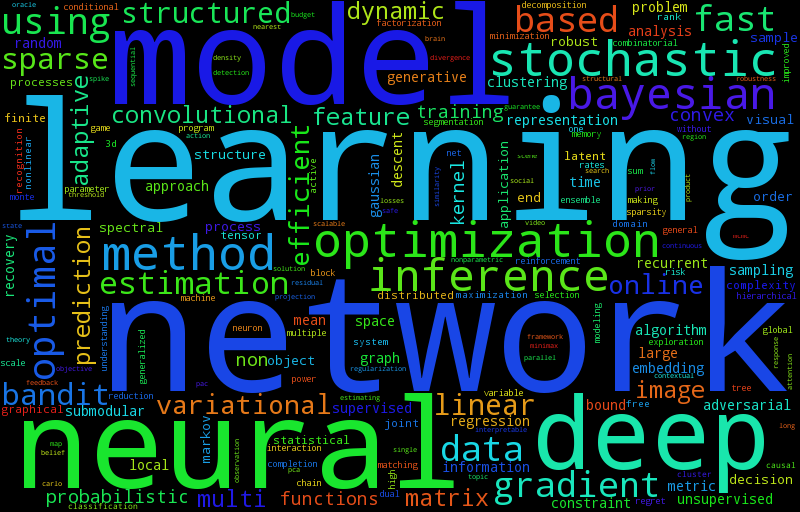
\includegraphics[height=2cm]{nipsWords.png}\hspace*{1.5cm}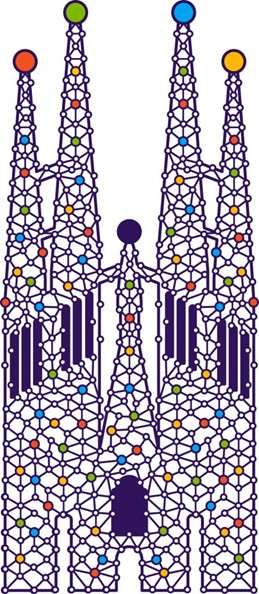
\includegraphics[height=2cm]{barcelonaLogo.jpg}}

\begin{document}

  \begin{frame}[noframenumbering]
    \titlepage
  \end{frame}

  \section{NIPS Conference}

  \subsection{History}

  \begin{frame}
    \frametitle{Neural Information Processing Systems}

    \begin{itemize}
      \item Largest International Conference on Machine Learning.
      \item Held since 1987 and focuses on AI, ML, Mathematics, Statistics.
    \end{itemize}

    \begin{figure}
      \centering
      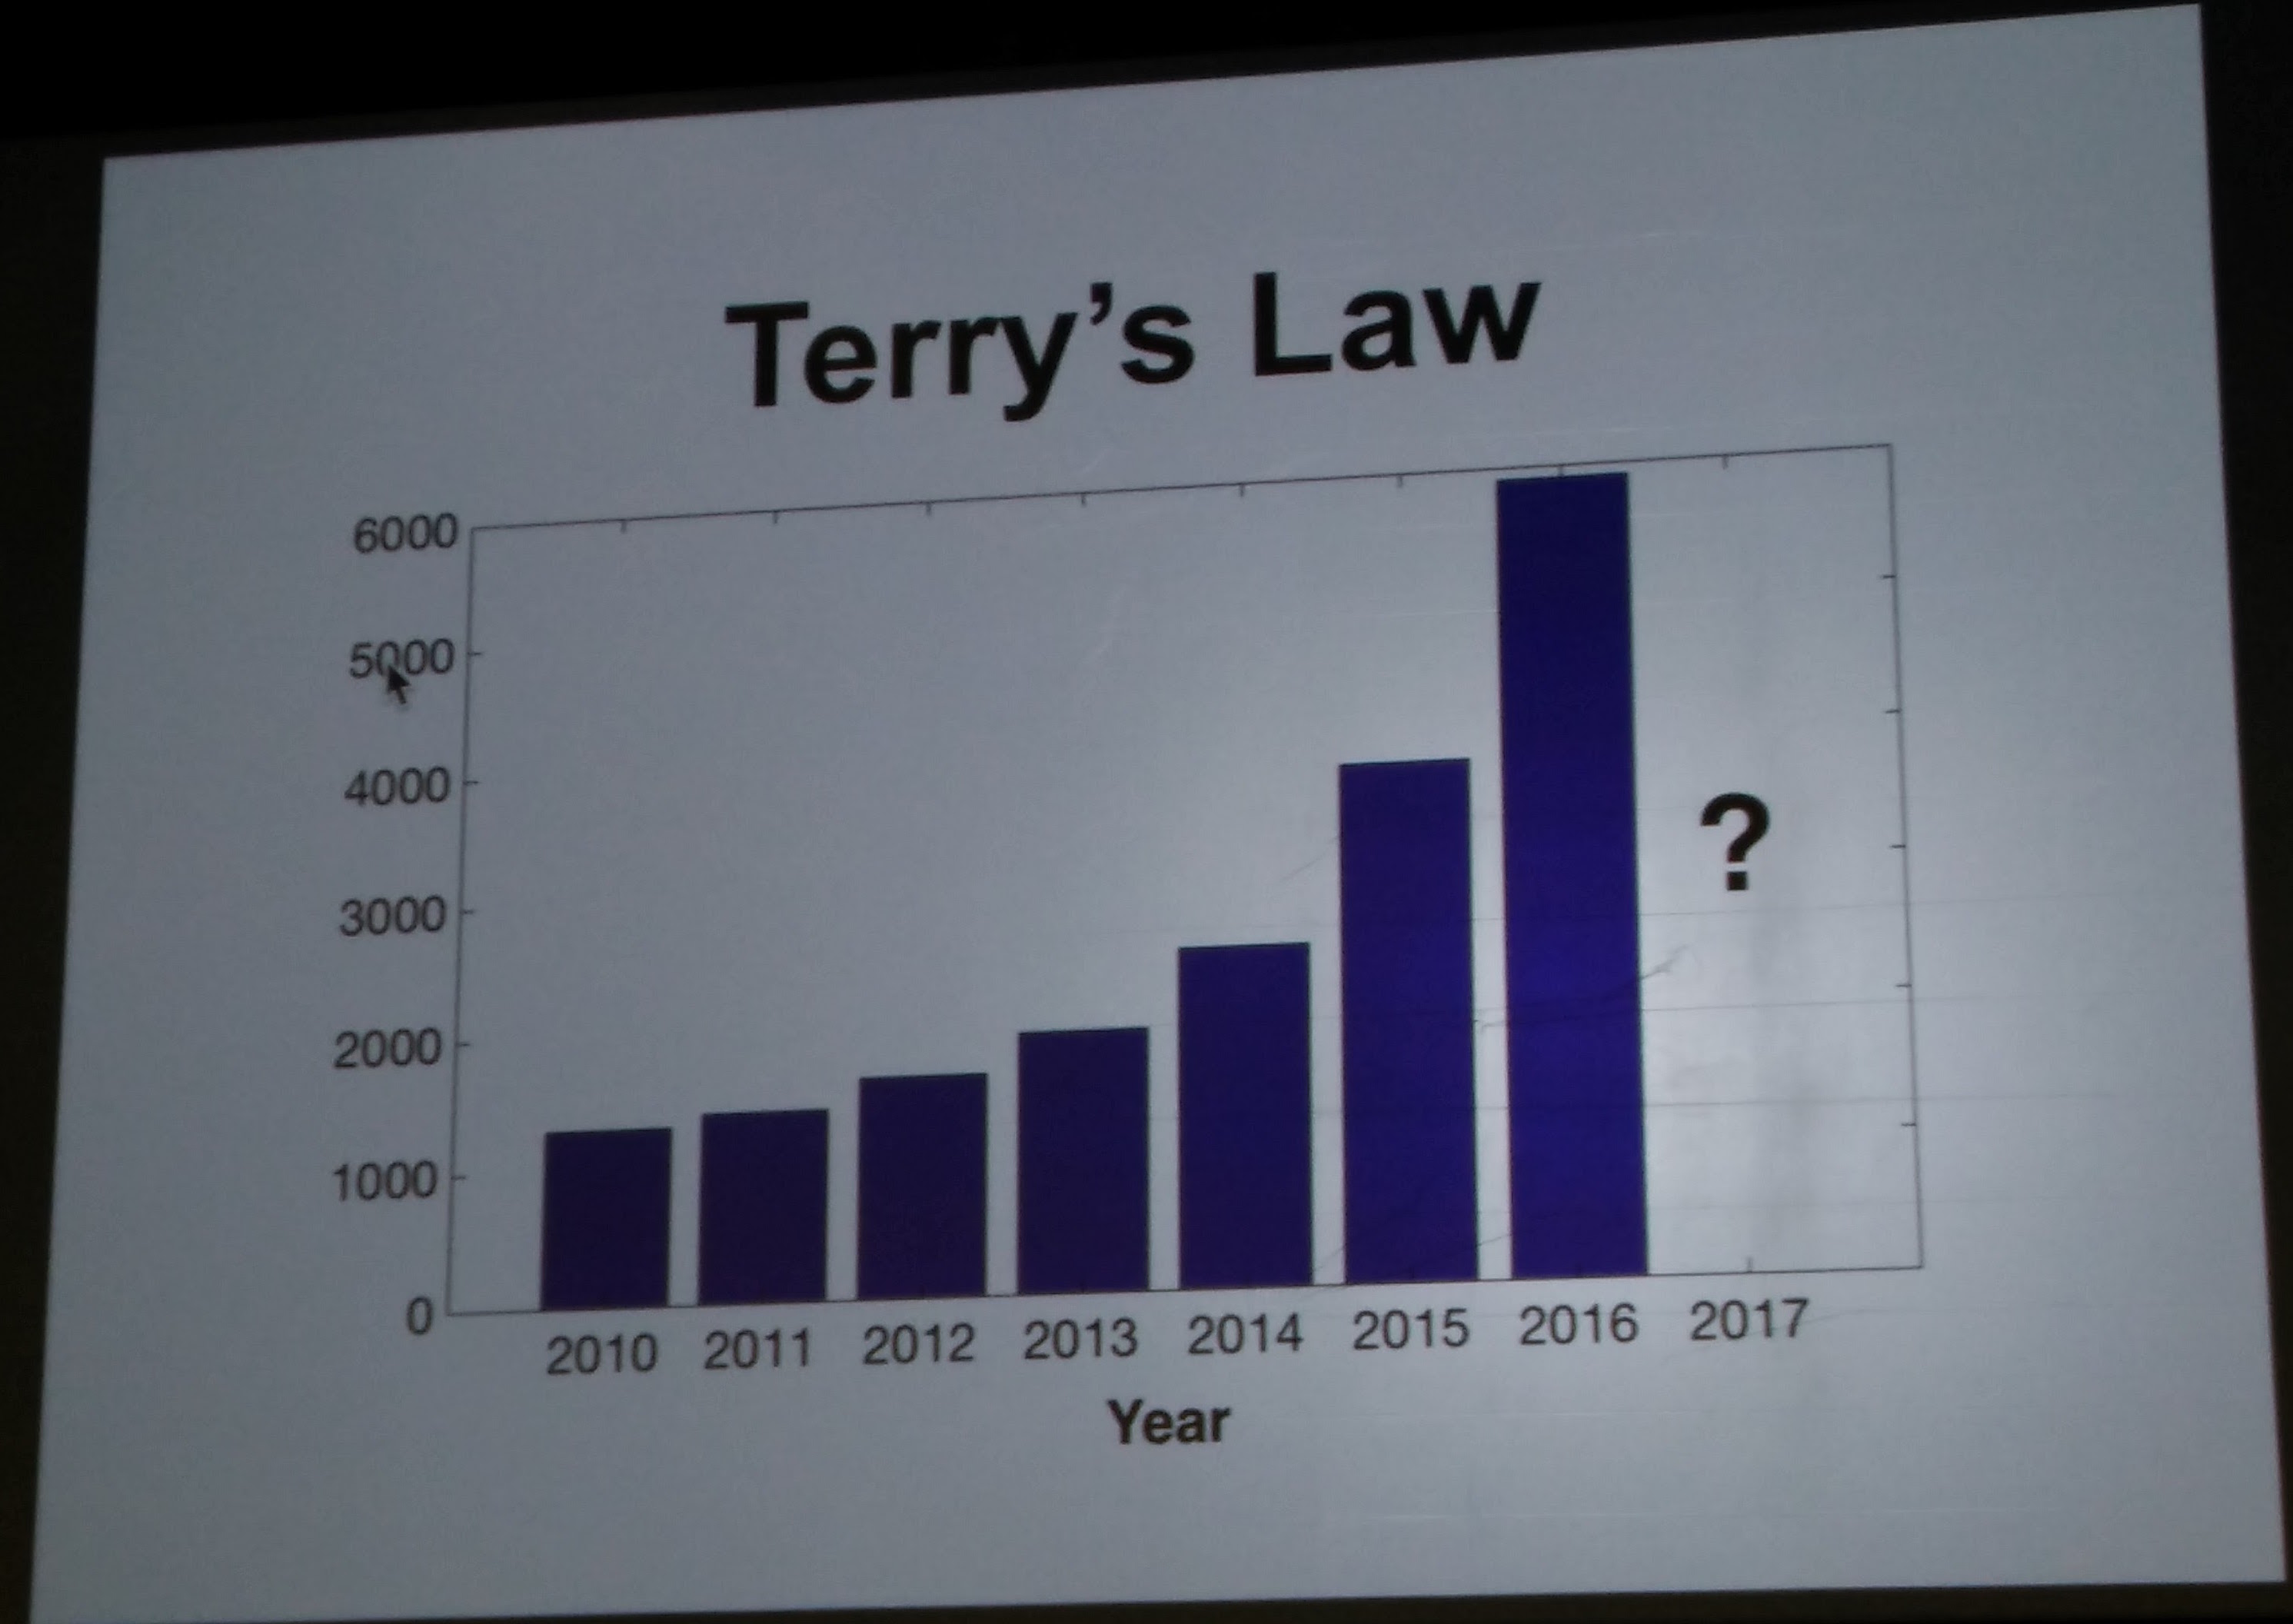
\includegraphics[width=0.65\textwidth]{terryLaw.jpg}
      \caption*{Terry's Law on NIPS Participants \footnotemark[1]}
    \end{figure}

    \footnotetext[1]{Proposed by \href{http://www.salk.edu/scientist/terrence-sejnowski/}{Terrence Sejnowski}, NIPS 2016 Chair}
  \end{frame}

  \subsection{Statistics}

  \begin{frame}
    \frametitle{NIPS 2016: Topics Convered}

    \begin{itemize}
      \item 568 Papers (46 oral) accepted among 2400 papers with 6 reviewers per submission.
      \item Most popular topics were Deep Learning (1 in 4) with application to Computer Vision (1 in 10).
    \end{itemize}

    \begin{figure}
      \centering
      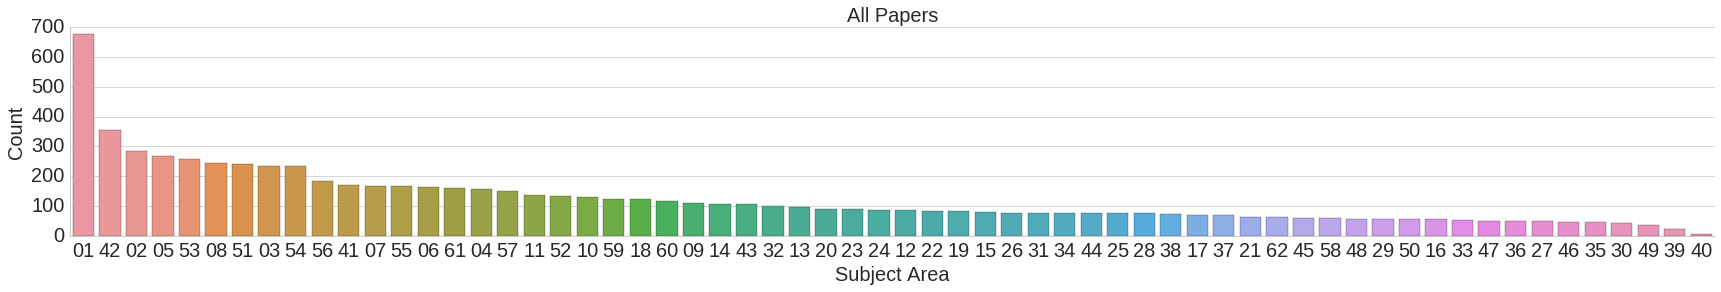
\includegraphics[width=\textwidth]{nipsTopics1.png}
    \end{figure}

    \begin{figure}
      \centering
      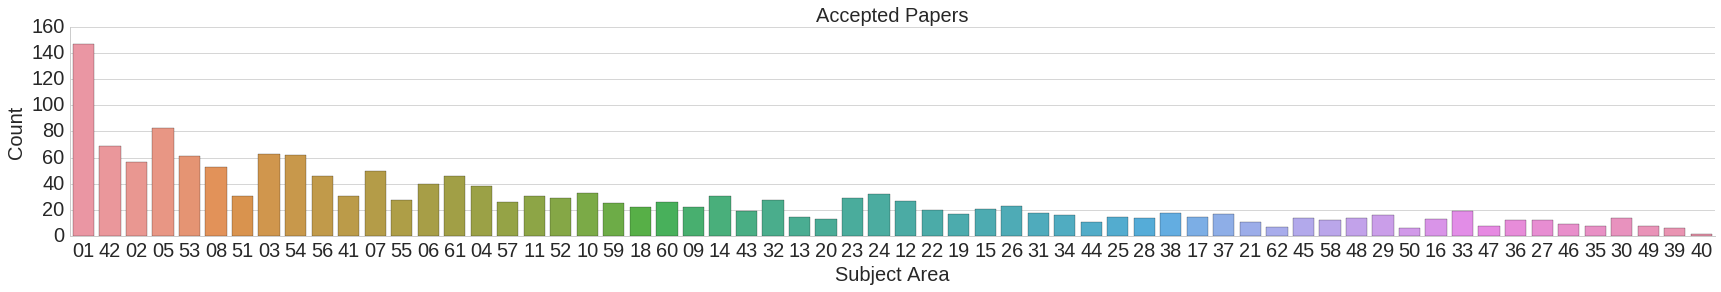
\includegraphics[width=\textwidth]{nipsTopics2.png}
      \caption*{Long-tailed Distribution of Topics \footnotemark[1]}
    \end{figure}

    \footnotetext[1]{\href{http://www.tml.cs.uni-tuebingen.de/team/luxburg/misc/nips2016/index.php}{NIPS 2016 Review Process}}
  \end{frame}

  \subsection{Impressions}

  \begin{frame}
    \frametitle{NIPS 2016: Impressions}

    \begin{itemize}
      \item \textbf{Strong industry presence}: Google Deepmind, Facebook AI Research, OpenAI etc
      \item \textbf{Philosophical panel discussions}: Healthy debates on general trends and future of community.
      \item \textbf{Emphasis on Deep Learning}: Studies on applications as well as \textbf{theoretical foundations} of Deep Learning.
    \end{itemize}
    \vskip-1em
    \begin{columns}
      \begin{column}{0.33\textwidth}
        \begin{figure}
          \centering
          \caption*{Tutorial on GANs\footnotemark[1]}
          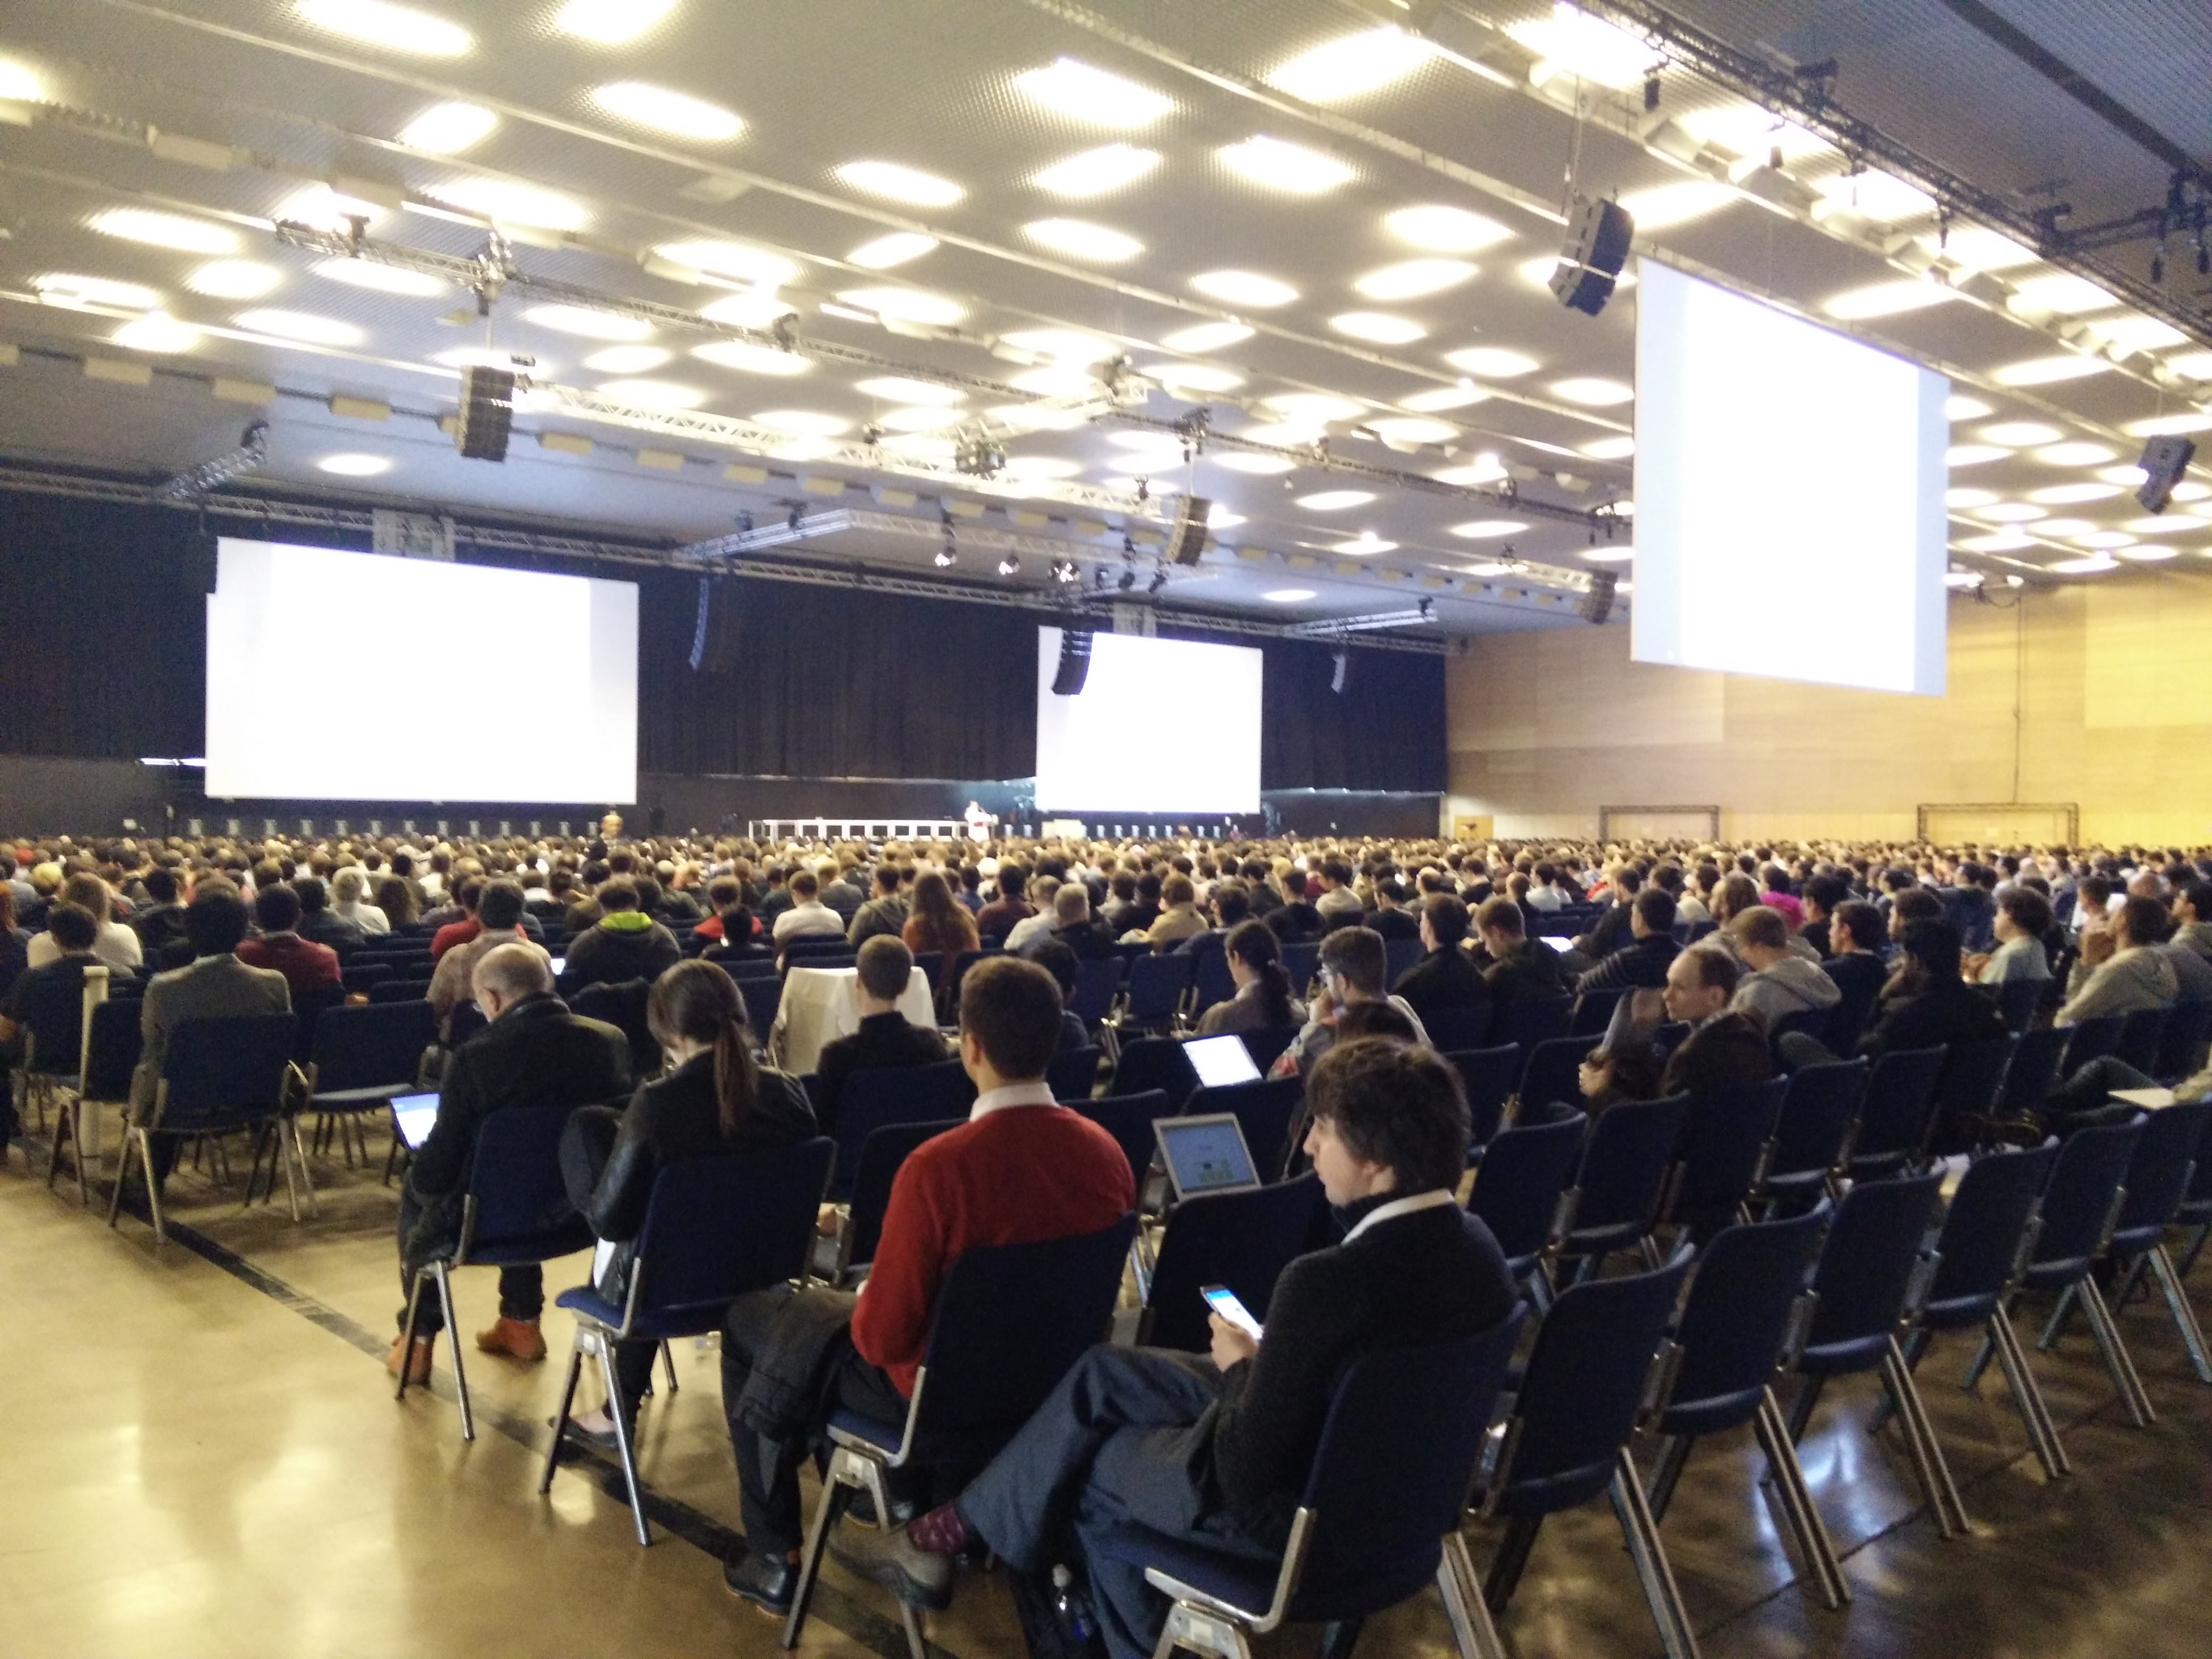
\includegraphics[width=\textwidth]{goodfellowTutorial.jpg}
        \end{figure}
      \end{column}
      \begin{column}{0.33\textwidth}
        \begin{figure}
          \centering
          \caption*{Conference Venue\footnotemark[1]}
          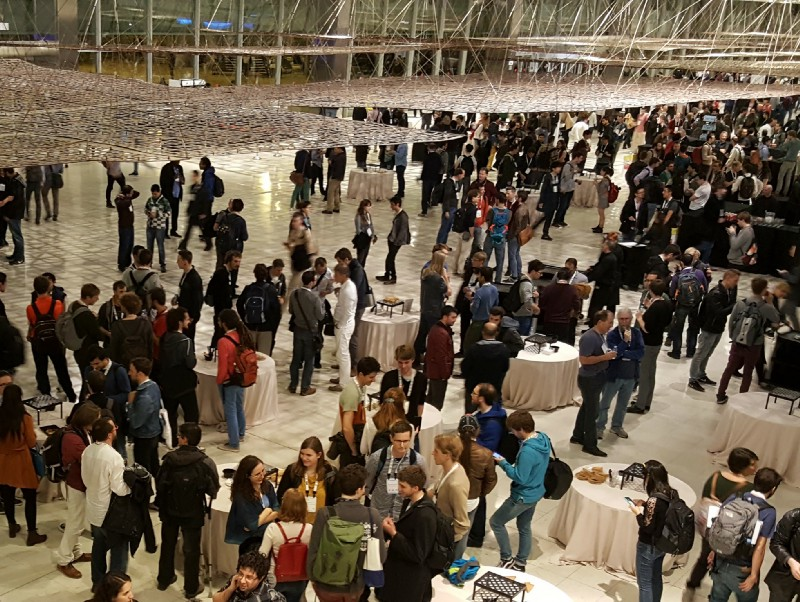
\includegraphics[width=\textwidth]{conferenceVenue.jpeg}
        \end{figure}
      \end{column}
      \begin{column}{0.33\textwidth}
        \begin{figure}
          \centering
          \caption*{Boston Dynamics\footnotemark[1]}
          \includegraphics[width=\textwidth]{bostonDyn.png}
        \end{figure}
      \end{column}
    \end{columns}

    \footnotetext[1]{\href{http://blog.aylien.com/wp-content/uploads/2016/12/full_conference_hall_gan_tutorial.jpg}{Ian Goodfellow's Tutorial on GAN}, \href{https://cdn-images-1.medium.com/max/800/1*l6ILYWwpF9A1KkqK6hwuaA.jpeg}{Image of Conference Venue}, \href{http://sebastianruder.com/content/images/2016/12/boston_dynamics_spot.png}{Boston Dynamics Spot Demo}}
  \end{frame}

  \section{General Topics}

  \begin{frame}
    \frametitle{Nuts and Bolts of ML: Andrew Ng}

    \begin{itemize}
      \item Practical advice on machine learning research
      \item Importance of human-level accuracy as metric
      \item Techniques for collecting data to train models.
    \end{itemize}

    \begin{figure}
      \centering
      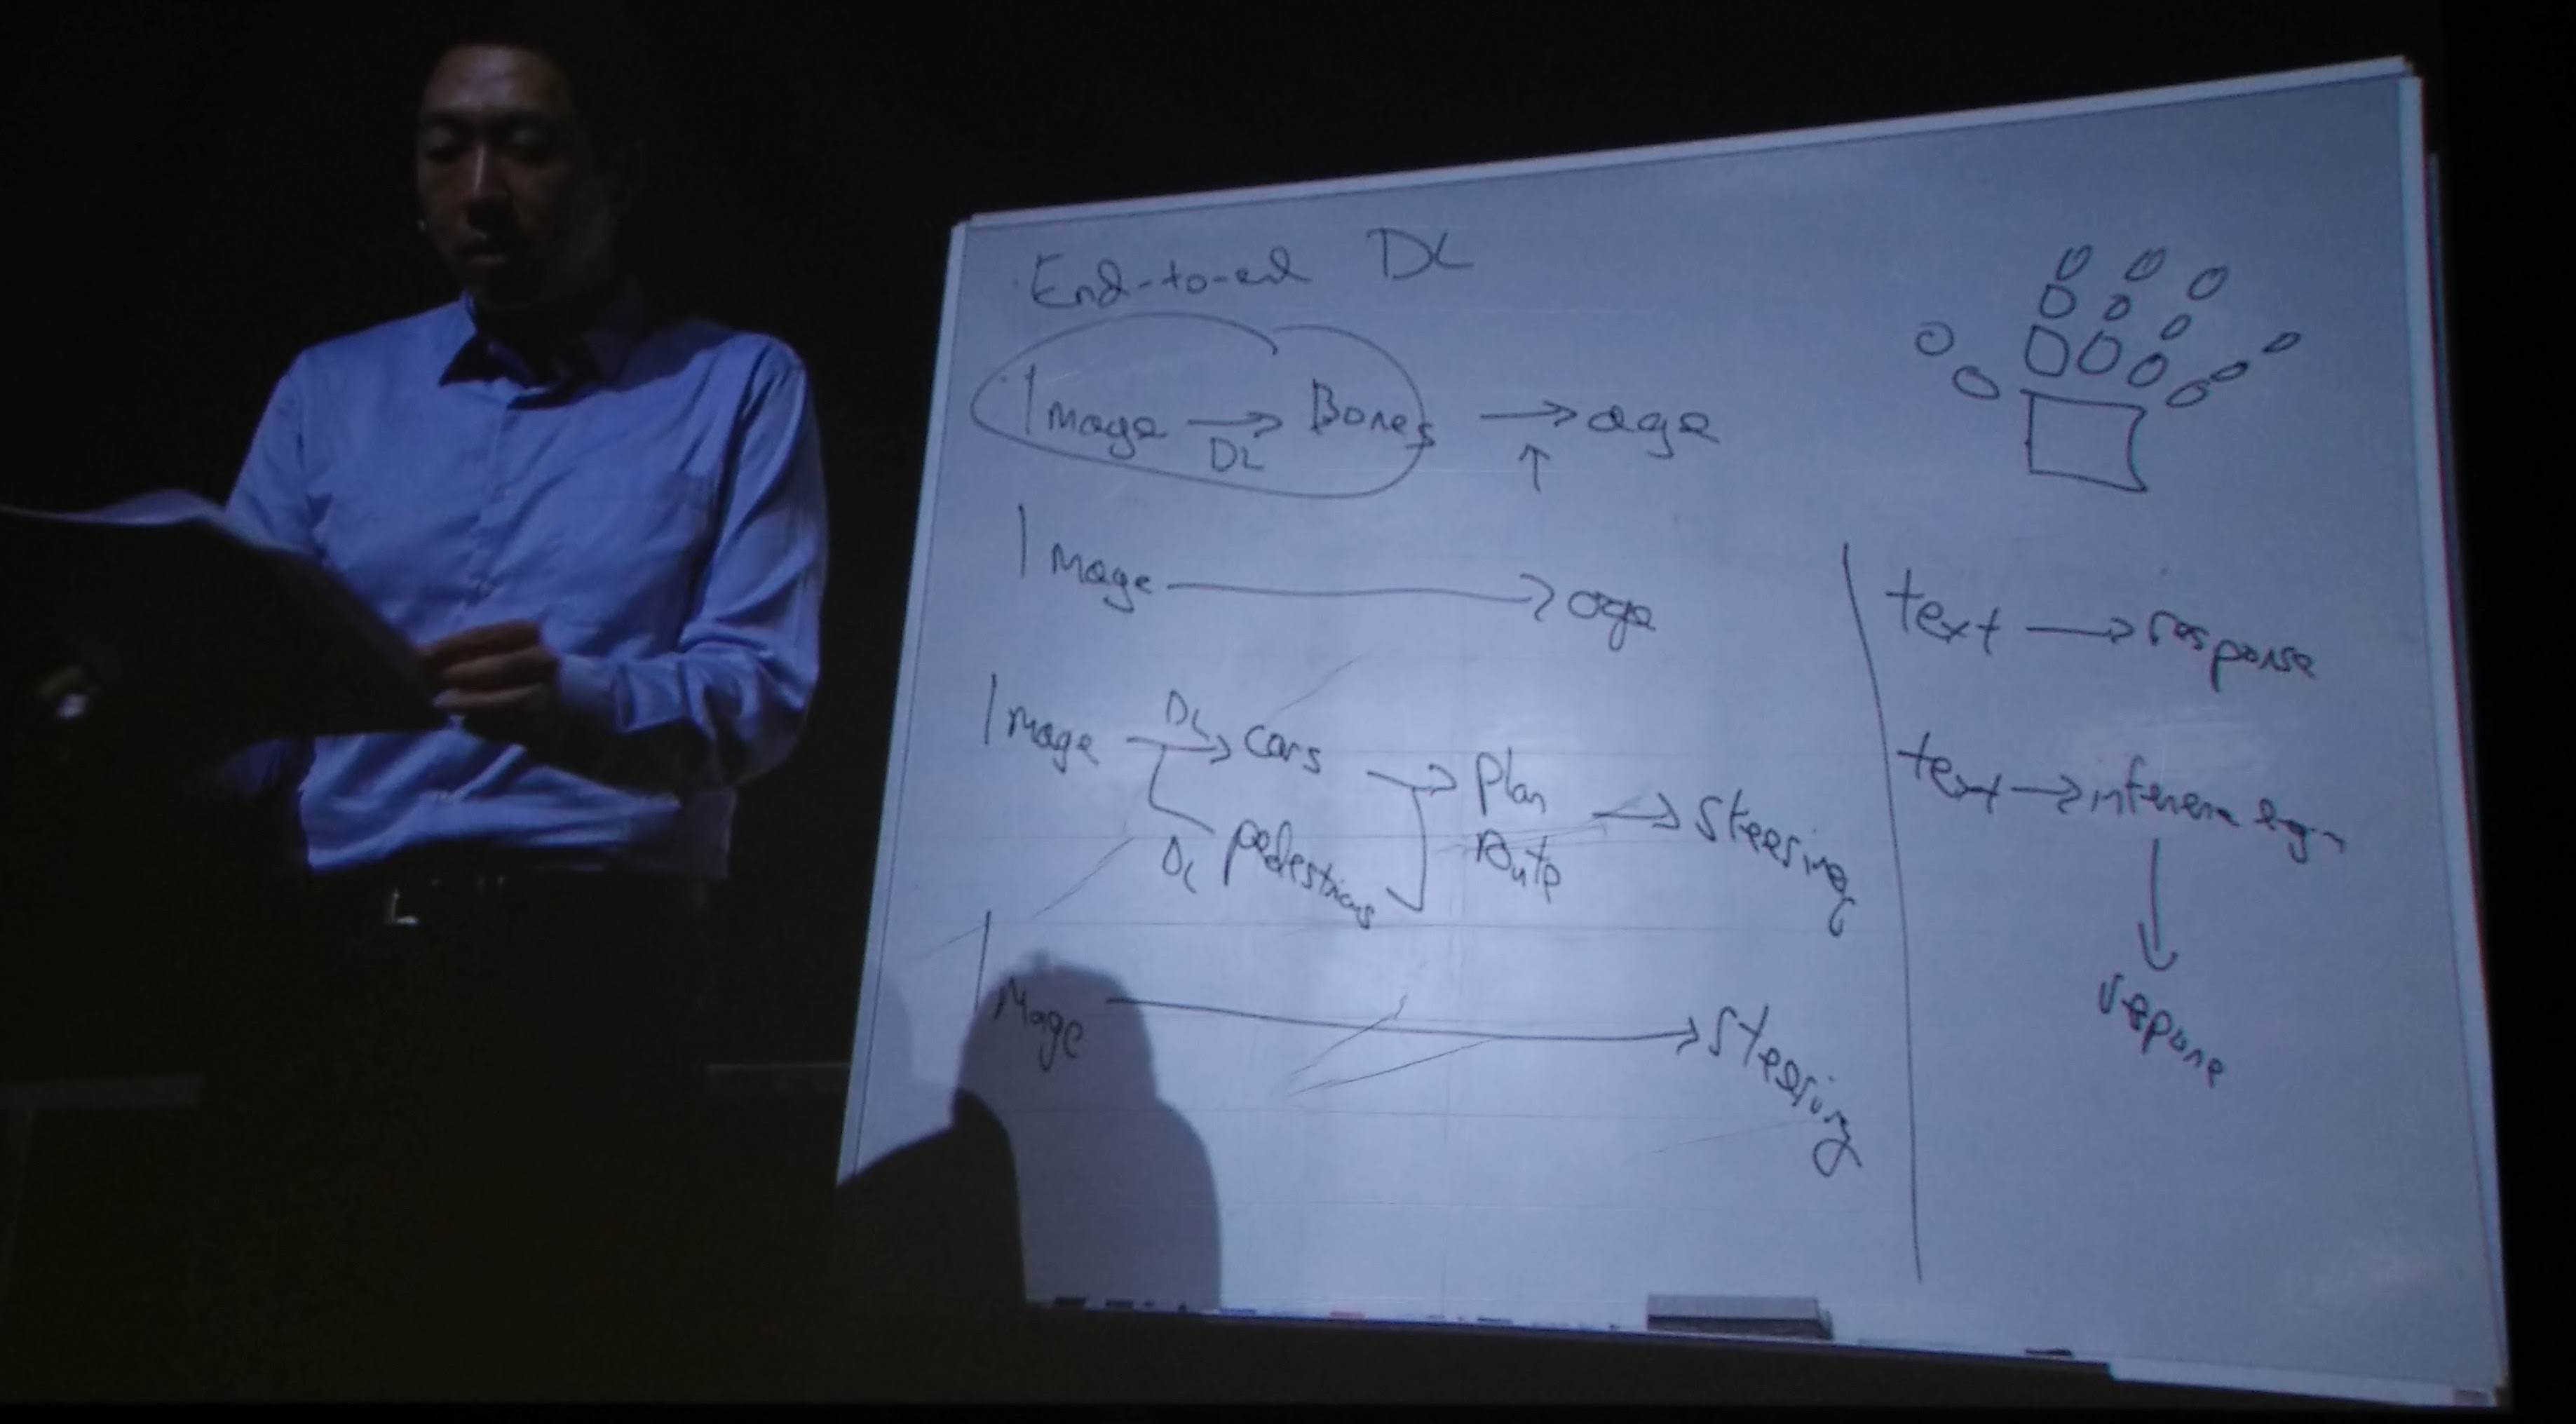
\includegraphics[width=0.8\textwidth]{ngKeynote.jpg}
    \end{figure}

    \footnotetext[1]{https://www.youtube.com/watch?v=F1ka6a13S9I}
  \end{frame}

  \begin{frame}
    \frametitle{Predictive Learning: Yann Lecun}

    \begin{figure}
      \centering
      \caption*{General AI means agents should have \textbf{Common Sense}\footnotemark[1]}
      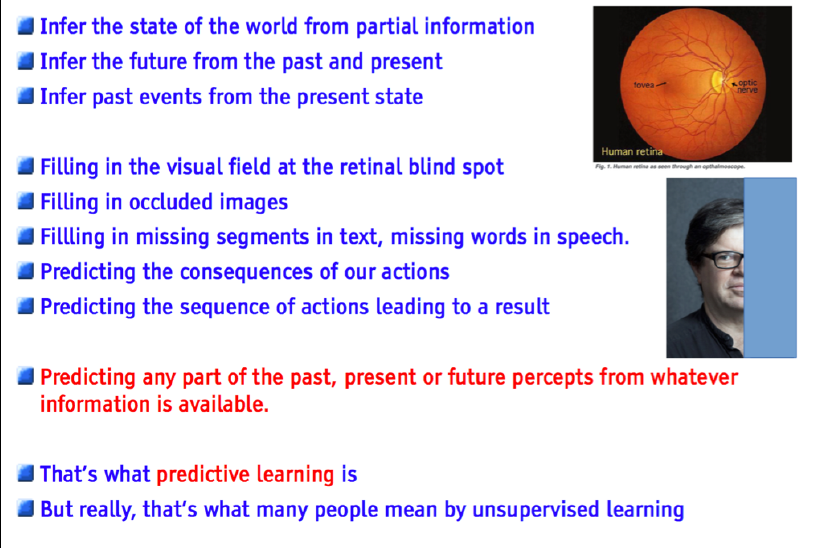
\includegraphics[width=0.8\textwidth]{generalAI2.png}
    \end{figure}

    \footnotetext[1]{\url{https://nips.cc/Conferences/2016/Schedule?showEvent=6197}}
  \end{frame}

  \begin{frame}
    \frametitle{Predictive Learning: Yann Lecun}

    \begin{figure}
      \centering
      \caption*{Key to General AI will be \textbf{Unsupervised Learning}\footnotemark[1]}
      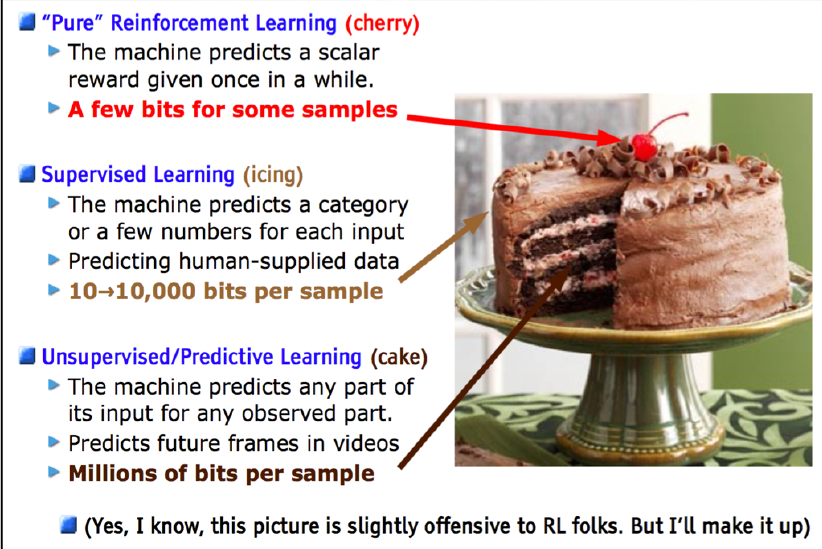
\includegraphics[width=0.8\textwidth]{generalAI1.png}
    \end{figure}

    \footnotetext[1]{\url{https://nips.cc/Conferences/2016/Schedule?showEvent=6197}}
  \end{frame}

  \begin{frame}
    \frametitle{Intelligent Biosphere: Drew Purves}

    \begin{figure}
      \centering
      \caption*{Intelligent life strongly depends on the environment and vice versa\footnotemark[1]}
      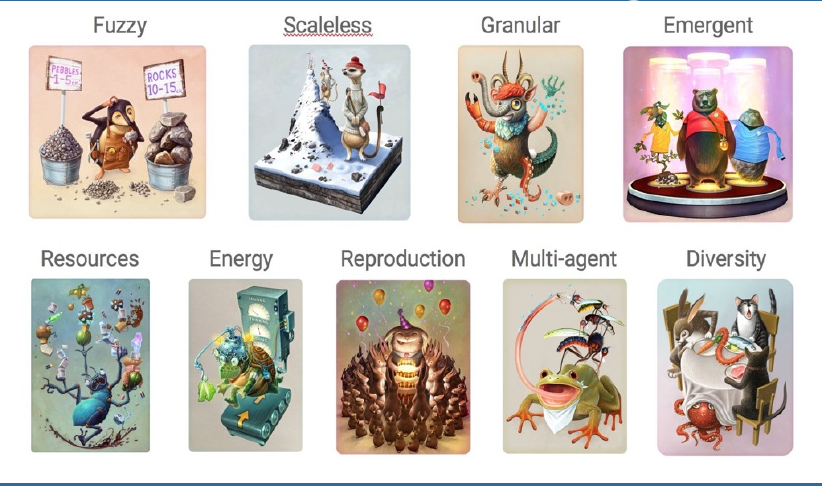
\includegraphics[width=0.8\textwidth]{generalAI4.png}
    \end{figure}

    \footnotetext[1]{\url{https://nips.cc/Conferences/2016/Schedule?showEvent=6193}}
  \end{frame}

  \begin{frame}
    \frametitle{Learning from the Brain: Saket Navlakha}

    \begin{figure}
      \centering
      \caption*{Pruning of neural connections is crucial for Learning in Brain\footnotemark[1]}
      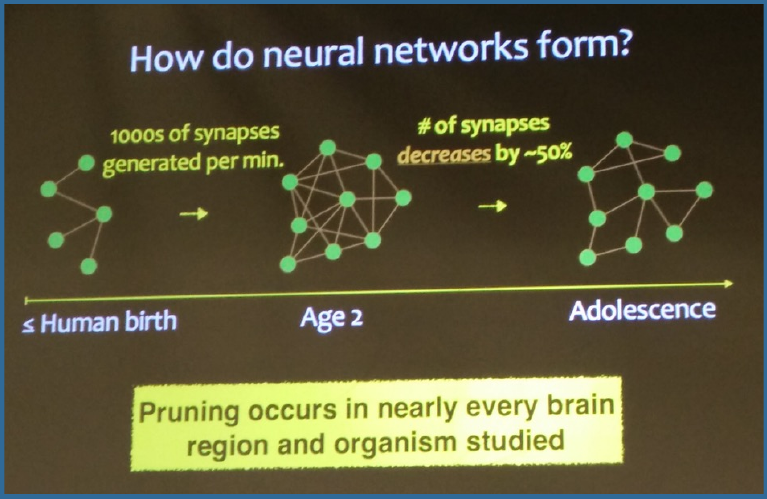
\includegraphics[width=0.8\textwidth]{generalAI3.png}
    \end{figure}

    \footnotetext[1]{https://nips.cc/Conferences/2016/Schedule?showEvent=6192}
  \end{frame}

  \section{Deep Learning}

  \subsection{Generative Adversarial Networks}

  \begin{frame}
    \frametitle{Generative Adversarial Networks: Overview}

    \begin{equation*}
      \text{min}_G~\text{max}_D~V(D,G) = \mathbb{E}_{x \sim p_{\text{data}}(x)} \log D(x) + \mathbb{E}_{x \sim p_{x}(z)} \log (1 - D(G(z)))
    \end{equation*}
    \vskip-1em
    \begin{figure}
      \centering
      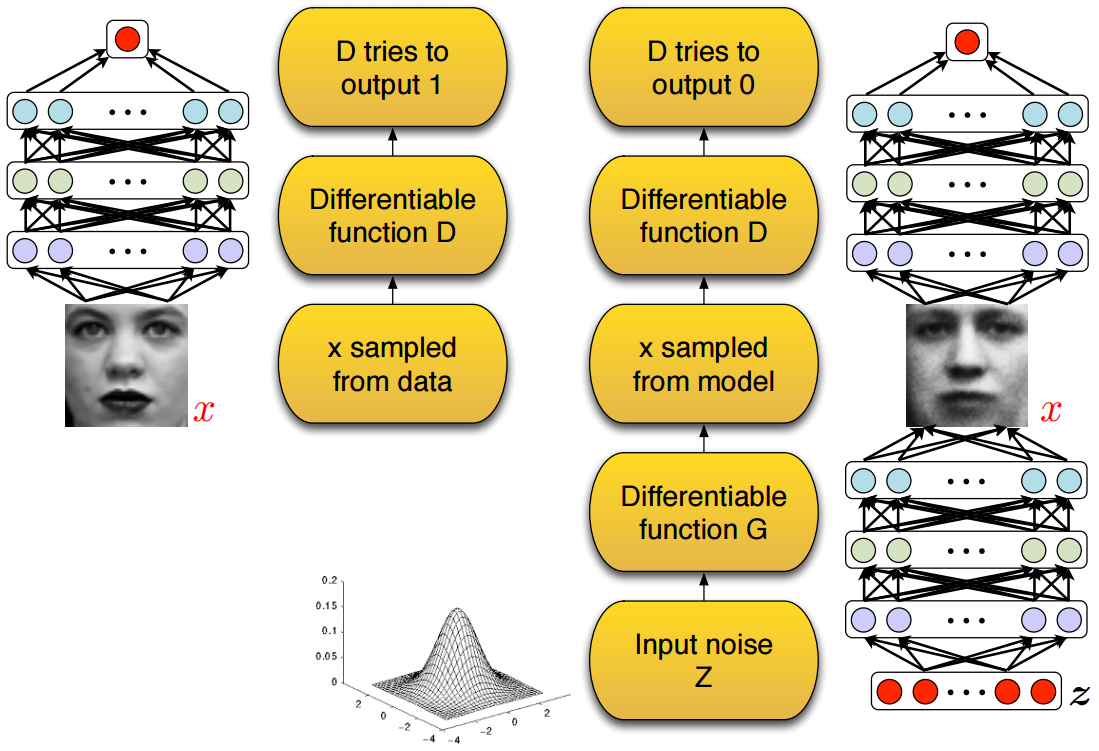
\includegraphics[width=0.75\textwidth]{gan1.png}
    \end{figure}

    \footnotetext[1]{Goodfellow et al. ``Generative adversarial nets'' in \emph{NIPS 2016}}
  \end{frame}

  \begin{frame}
    \frametitle{GAN: Tutorials}

    \begin{itemize}
      \item \href{http://www.iangoodfellow.com/slides/2016-12-04-NIPS.pdf}{Tutorial on GANs by Ian Goodfellow}:
        \begin{itemize}
          \item Applications to generate realistic images.
          \item Learn latent manifolds encoding task variability.
          \item Theoretical challenges for training models.
        \end{itemize}
      \item \href{https://github.com/soumith/ganhacks}{Tutorial on Practical Tips by Soumith Chintala}:
        \begin{itemize}
          \item Tips on data preprocessing, network design and optimizers.
        \end{itemize}
    \end{itemize}
    \vskip-1em
    \begin{columns}
      \begin{column}{0.33\textwidth}
        \begin{figure}
          \centering
          \caption*{Manifold on MNIST\footnotemark[1]}
          
\includegraphics[width=0.9\textwidth]{gan2.png}
        \end{figure}
      \end{column}
      \begin{column}{0.33\textwidth}
        \begin{figure}
          \centering
          \caption*{Tutorial by Chintala\footnotemark[1]}
          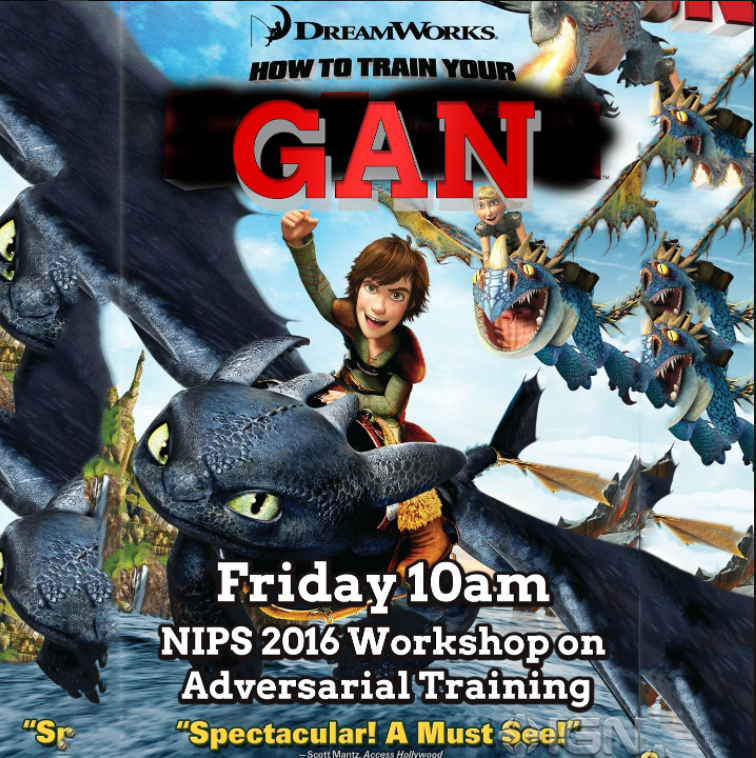
\includegraphics[width=0.9\textwidth]{chintalaTutorial.png}
        \end{figure}
      \end{column}
    \end{columns}

    \footnotetext[1]{\href{http://www.iro.umontreal.ca/~bengioy/talks/dlss-12aug2015.pdf}{Presentation at DLSS 2015}, \href{https://github.com/soumith/ganhacks}{How to Train Your GAN}}
  \end{frame}

  \begin{frame}
    \frametitle{GAN: Applications}

    \begin{columns}
      \begin{column}{0.5\textwidth}
        \centering
        Learning What and Where\footnotemark[1]

        \begin{figure}
          \centering
          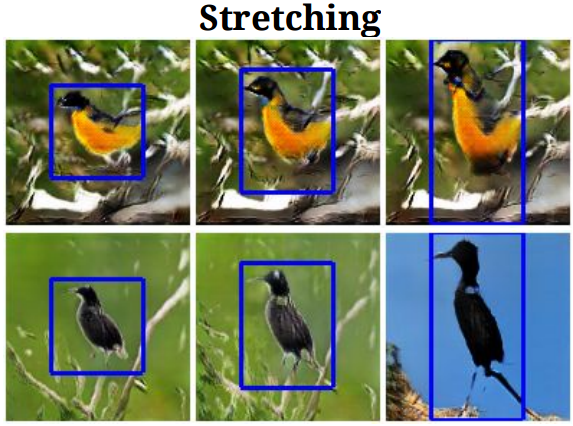
\includegraphics[width=0.75\textwidth, height=0.25\textheight]{ganApp1.png}
        \end{figure}
        \vskip-1em
        \begin{itemize}
          \item Use text input to generate novel images.
          \item Architecture for location and content controllable synthesis.
        \end{itemize}
      \end{column}

      \begin{column}{0.5\textwidth}
        \centering
        Information Maximizing GANs\footnotemark[2]

        \begin{figure}
          \centering
          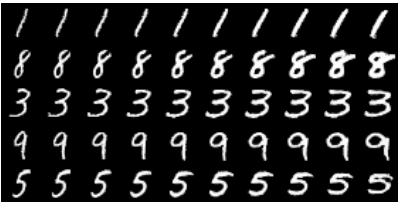
\includegraphics[width=0.9\textwidth]{ganApp2.png}
        \end{figure}
        \vskip-1em
        \begin{itemize}
          \item Unsupervised learning of \textbf{disentagled} representations.
          \item Maximizes mutual information between latent variables and observations.
        \end{itemize}
      \end{column}
    \end{columns}

    \footnotetext[1]{Reed et al., ``Learning what and where to draw'' in \emph{NIPS 2016}}
    \footnotetext[2]{Chen et al., ``Infogan: Interpretable representation learning by information maximizing generative adversarial nets'' in \emph{NIPS 2016}}
  \end{frame}

  \subsection{Bayesian Deep Learning}

  \begin{frame}
    \frametitle{Bayesian Deep Learning}

    \begin{itemize}
      \item \href{http://bayesiandeeplearning.org/slides/nips16bayesdeep.pdf}{History of Bayesian Neural Networks by Zoubin Gharamani\footnotemark[1]}:
        \begin{itemize}
          \item Derives from Gaussian Process Regression
          \item Feature selection possible using Automatic Relevance Determination
          \item Current research on variational inference techniques
        \end{itemize}
    \end{itemize}

    \begin{figure}
      \centering
      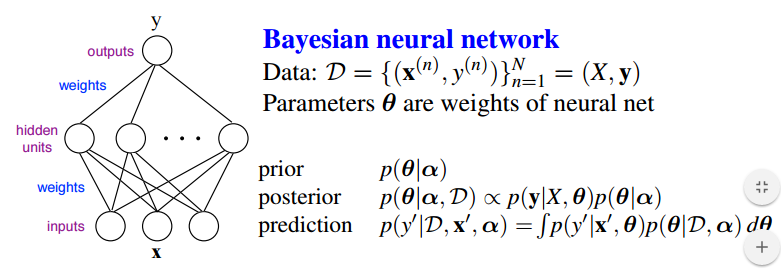
\includegraphics[width=\textwidth]{bnn1.png}
    \end{figure}

    \footnotetext[1]{Keynote Talk by Zoubin Gharamani}
  \end{frame}

  \begin{frame}
    \frametitle{Deep Learning and Graphical Models}

    \centering Combined training of Graphical Models and Deep Neural Networks using Variational Inference\footnotemark[1]

    \begin{figure}
      \centering
      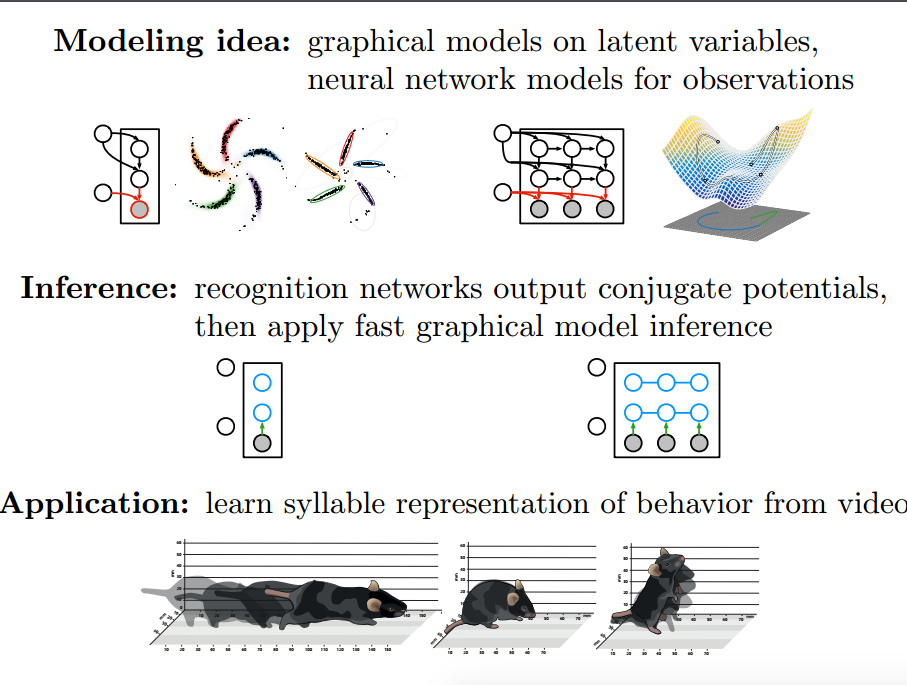
\includegraphics[width=0.75\textwidth]{bnn2.png}
    \end{figure}

    \footnotetext[1]{Johnson et al., ``Composing graphical models with neural networks for structured representations and fast inference'' in \emph{NIPS 2016}}
  \end{frame}

  \begin{frame}
    \frametitle{Dropout as a Bayesian Approximation}

    \centering Dropout is equivalent to variational inference in Deep GPs with specific kernel function

    \begin{figure}
      \centering
      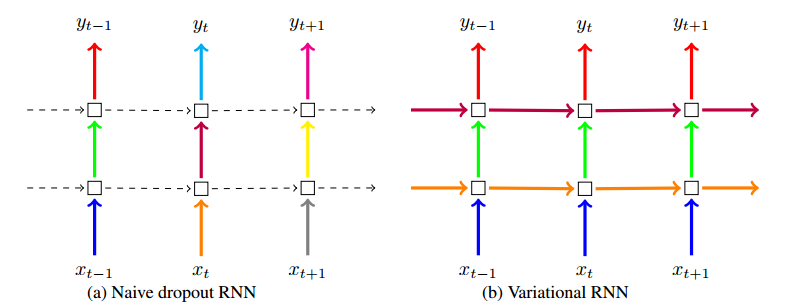
\includegraphics[width=\textwidth]{bnn4.png}
    \end{figure}

    \footnotetext[1]{Gal et al., ``A theoretically grounded application of dropout in recurrent neural networks'' in \emph{NIPS 2016}}
  \end{frame}

  \subsection{Deep Reinforcement Learning}

  \begin{frame}
    \frametitle{Deep Reinforcement Learning: Tutorials}

    \begin{itemize}
      \item \href{http://people.eecs.berkeley.edu/~pabbeel/nips-tutorial-policy-optimization-Schulman-Abbeel.pdf}{Deep RL through Policy Optimization\footnotemark[1]}:
        \begin{itemize}
          \item History of policy search RL focusing on Deep RL
          \item Future work on \textbf{Skill Transfer} and \textbf{Exploration}
        \end{itemize}
      \item \href{http://rll.berkeley.edu/deeprlcourse/docs/nuts-and-bolts.pdf}{Nuts and Bolts of Deep RL Research\footnotemark[2]}:
        \begin{itemize}
          \item Tips on implementing existing algorithms
          \item Problem formulation for novel tasks
        \end{itemize}
    \end{itemize}

    \begin{figure}
      \centering
      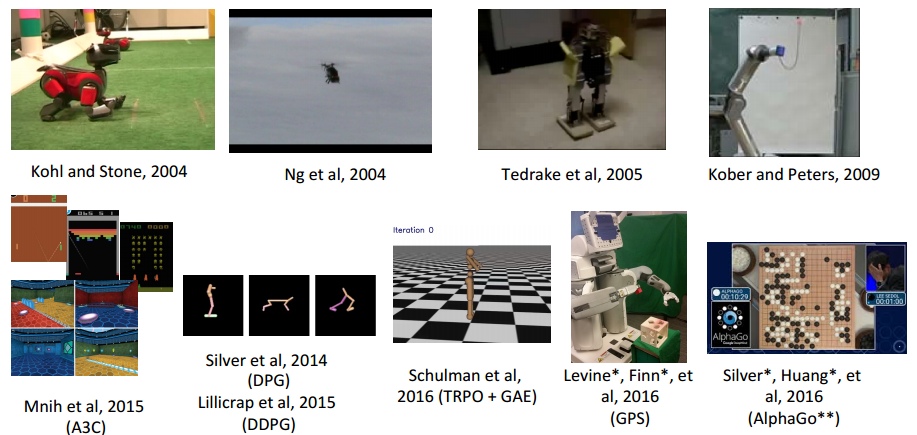
\includegraphics[width=0.8\textwidth]{drl1.png}
    \end{figure}

    \footnotetext[1]{Tutorial by Pieter Abbeel and John Schulman}
    \footnotetext[2]{Tutorial by John Schulman in Deep RL Workshop}
  \end{frame}

  \begin{frame}
    \frametitle{Opensource Environments}

    \begin{itemize}
      \item OpenAI Universe\footnotemark[1]: Develop and implement RL algorithms on many environments.
      \item Google Deepmind\footnotemark[2]: Simulator of 3D environments such as \textbf{Quake} and puzzle tasks.
      \item Facebook TorchCraft\footnotemark[3]: Bridge between Torch Library and Starcraft Game.
    \end{itemize}
    \vskip-1.5em
    \begin{columns}
      \begin{column}{0.33\textwidth}
        \begin{figure}
          \centering
          \caption*{OpenAI Universe}
          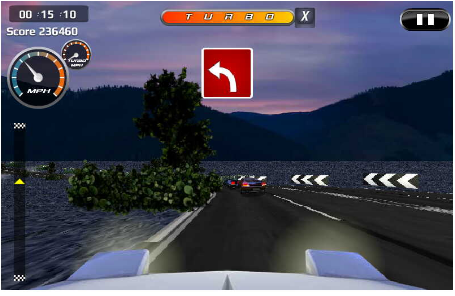
\includegraphics[width=0.8\textwidth]{drlApp1.png}
        \end{figure}
      \end{column}
      \begin{column}{0.33\textwidth}
        \begin{figure}
          \centering
          \caption*{Google Deepmind}
          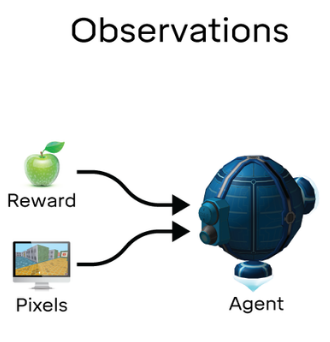
\includegraphics[width=0.8\textwidth, height=0.25\textheight]{drlApp2.png}
        \end{figure}
      \end{column}
      \begin{column}{0.33\textwidth}
        \begin{figure}
          \centering
          \caption*{Facebook Starcraft}
          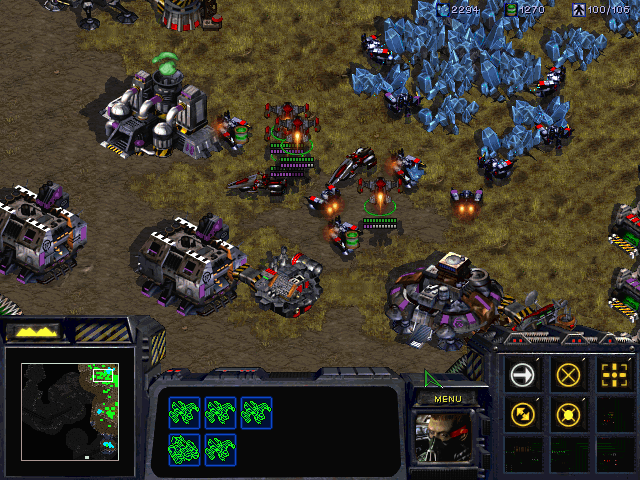
\includegraphics[width=0.8\textwidth]{drlApp3.png}
        \end{figure}
      \end{column}
    \end{columns}

    \footnotetext[1]{\href{https://openai.com/blog/universe/}{OpenAI Universe Press Release}}
    \footnotetext[2]{\href{https://deepmind.com/blog/open-sourcing-deepmind-lab/}{Google Deepmind Blog}}
    \footnotetext[3]{\href{https://github.com/TorchCraft/TorchCraft}{TorchCraft Repository on Github}}
  \end{frame}

  \begin{frame}
    \frametitle{Value Iteration Networks: Best Paper Award}

    \centering
    Represent Bellman equations with Convolutional Neural Networks to learn Value function
    \begin{figure}
      \centering
      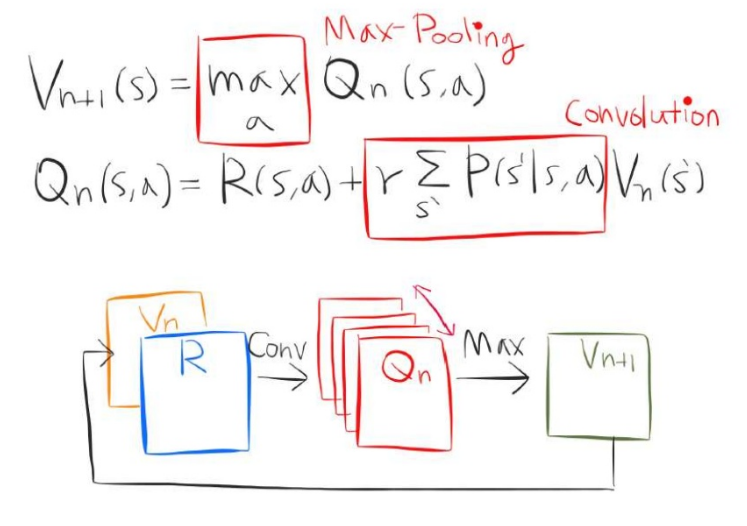
\includegraphics[width=0.8\textwidth]{drl2.png}
    \end{figure}

    \footnotetext[1]{Tamar et al., ``Value Iteration Networks'' in \emph{NIPS 2016}}
  \end{frame}

  \subsection{Recurrent Neural Networks}

  \begin{frame}
    \frametitle{Recurrent Neural Networks: Overview}

    \begin{itemize}
      \item Papers on theoretical foundations (\textbf{better architectures}\footnotemark[1]) and applications (\textbf{Reinforcement Learning}\footnotemark[2]).
      \item Strong correspondence to Neuroscience research (Fast and Slow time scales\footnotemark[3]).
    \end{itemize}

    \begin{figure}
      \centering
      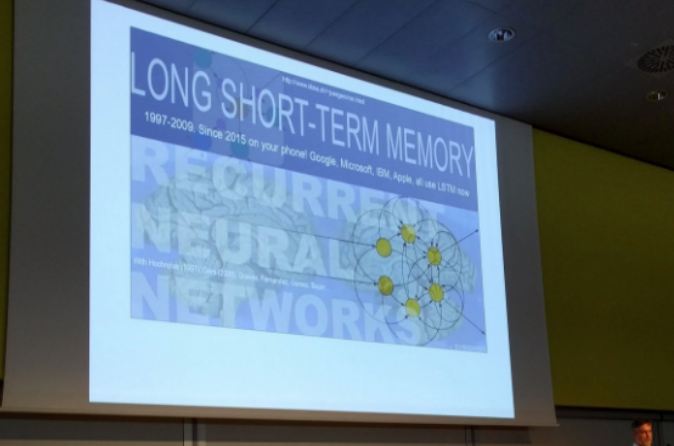
\includegraphics[width=0.7\textwidth,height=0.45\textheight]{rnn2.png}
    \end{figure}

    \footnotetext[1]{http://papers.nips.cc/paper/6114-weight-normalization-a-simple-reparameterization-to-accelerate-training-of-deep-neural-networks}
    \footnotetext[2]{https://arxiv.org/pdf/1611.02779.pdf}
    \footnotetext[3]{http://papers.nips.cc/paper/6310-phased-lstm-accelerating-recurrent-network-training-for-long-or-event-based-sequences}
  \end{frame}

  \subsection{Meta-learning}

  \begin{frame}
    \frametitle{Learning to (learn by gradient descent) by gradient descent}

    \begin{itemize}
      \item Current optimizers are parametric and domain specific.
      \item Attempt to learn the optimizer using RNN.
    \end{itemize}
    \begin{equation}
      \theta_{t+1} := \theta_t + g(\Delta f(\theta_t), \phi)
    \end{equation}

    \begin{figure}
      \centering
      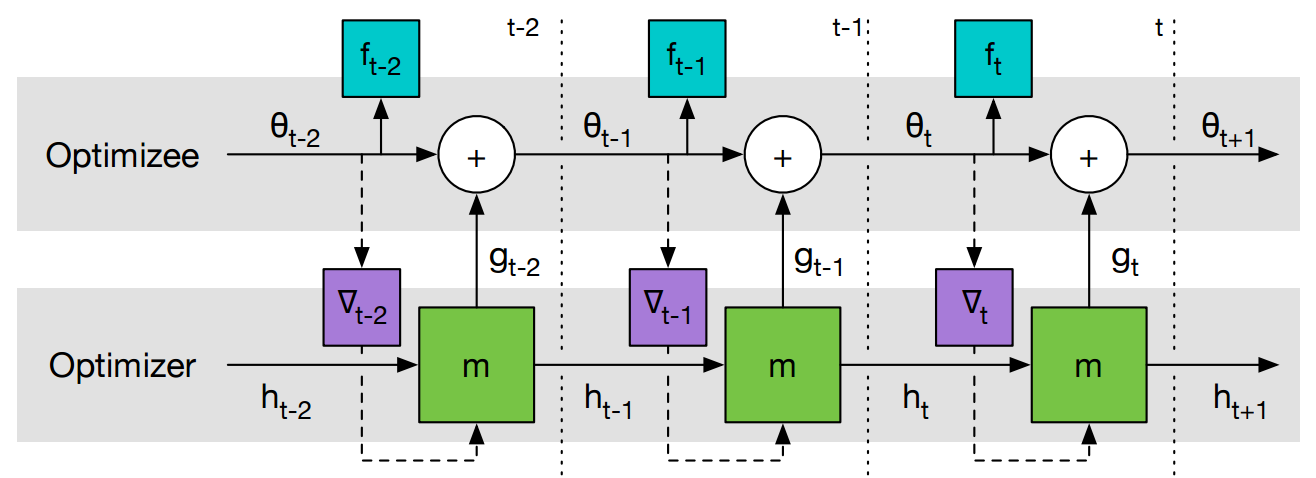
\includegraphics[width=0.9\textwidth]{metalearning1.png}
    \end{figure}

    \footnotetext[1]{Andrychowicz et al., ``Learning to learn by gradient descent by gradient descent'' in \emph{NIPS 2016}}
  \end{frame}

  \begin{frame}
    \frametitle{One-shot Learning}

    \begin{itemize}
      \item Novel architectures proposed for one-shot learning.
      \item The idea is a differentiable nearest neighbor classifier.
    \end{itemize}

    \begin{figure}
      \centering
      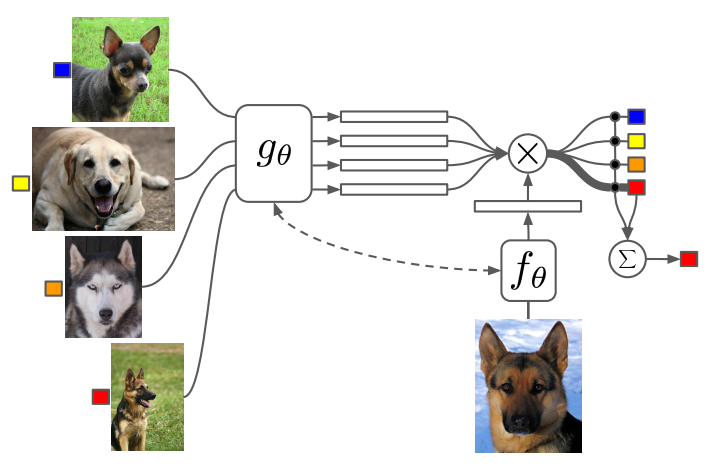
\includegraphics[width=0.8\textwidth]{oneshot1.png}
    \end{figure}

    \footnotetext[1]{Vinyals et al., ``Matching networks for one shot learning'' in \emph{NIPS 2016}}
  \end{frame}

  \subsection{Differentiable Neural Computers}

  \begin{frame}
    \frametitle{Differentiable Neural Computers}

    \begin{itemize}
      \item Neural Network with memory access (Read, Write, Link).
      \item Used for skill transfer, reinforcement learning, reasoning etc.
    \end{itemize}

    \begin{figure}
      \centering
      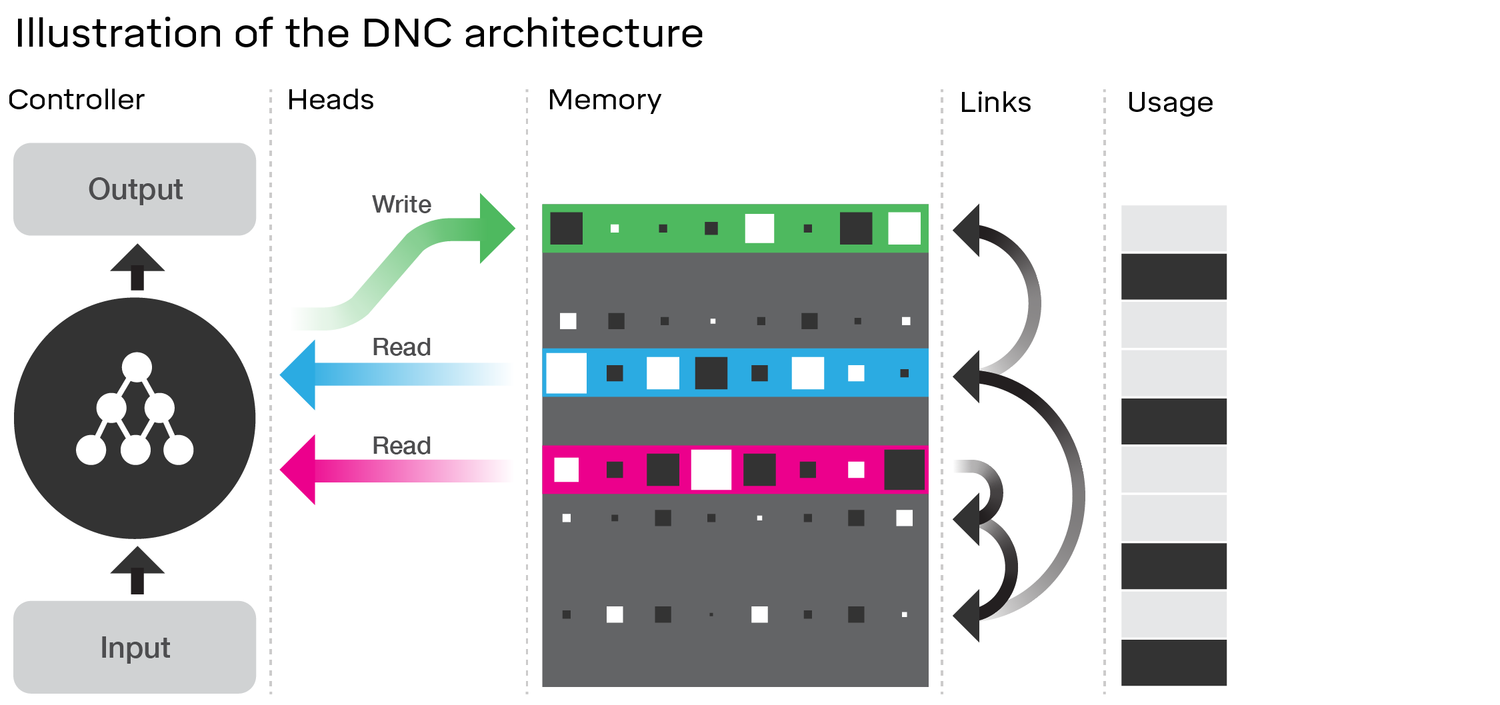
\includegraphics[width=0.8\textwidth]{dnc.png}
    \end{figure}

    \footnotetext[1]{https://deepmind.com/blog/differentiable-neural-computers/}
  \end{frame}

  \section{Other Topics}

  \begin{frame}
    \frametitle{Boston Robotics Demo}

    \begin{center}
      \href{run:./Videos/BostonDyn.avi?loop}{\includegraphics[width=0.9\textwidth]{./Videos/BostonDyn.png}}
    \end{center}

    \footnotetext[1]{https://nips.cc/Conferences/2016/Schedule?showEvent=6194}
  \end{frame}

  \begin{frame}
    \frametitle{Classic Algorithms: KMeans and Matrix Completion}

    \begin{itemize}
      \item Matrix completion: Non-convex objective for matrix completion has no spurious local minima \footnotemark[1]
      \item Clustering: Seedings for large-scale k-means++ clustering \footnotemark[2]
    \end{itemize}

    \begin{figure}
      \centering
      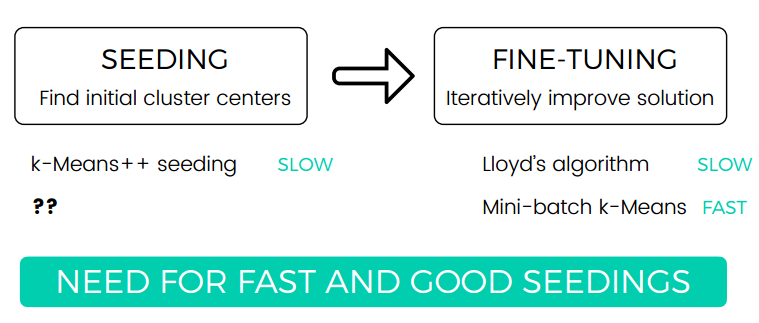
\includegraphics[width=0.9\textwidth]{kmeans.png}
    \end{figure}

    \footnotetext[1]{http://papers.nips.cc/paper/6048-matrix-completion-has-no-spurious-local-minimum}
    \footnotetext[2]{http://papers.nips.cc/paper/6478-fast-and-provably-good-seedings-for-k-means}
  \end{frame}

  \begin{frame}
    \frametitle{RocketAI: The AI Bubble}

    \centering Prank by NIPS organizers to warn about the AI Bubble

    \begin{figure}
      \centering
      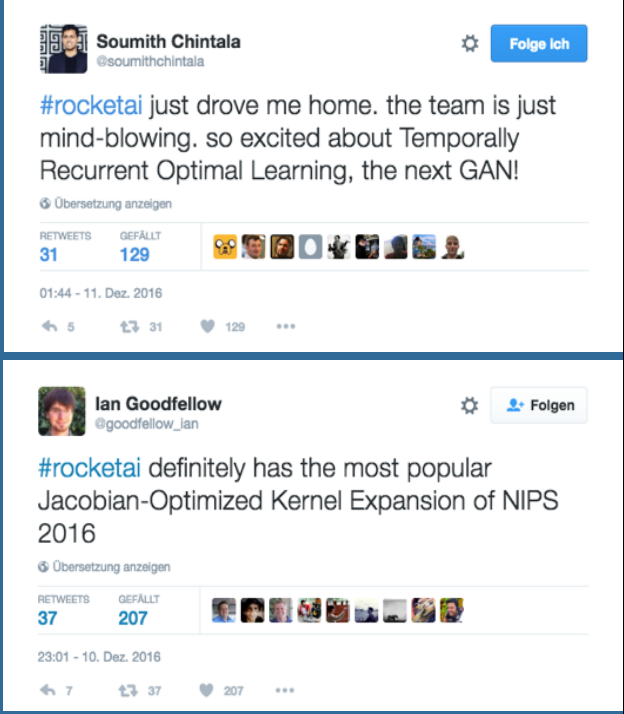
\includegraphics[width=0.5\textwidth]{rocketai2.png}
    \end{figure}

    \footnotetext[1]{\url{https://medium.com/the-mission/rocket-ai-2016s-most-notorious-ai-launch-and-the-problem-with-ai-hype-d7908013f8c9}}
  \end{frame}


  \begin{frame}
    \frametitle{Sightseeing in Barcelona}

    \begin{columns}
      \begin{column}{0.5\textwidth}
        \begin{figure}
          \centering
          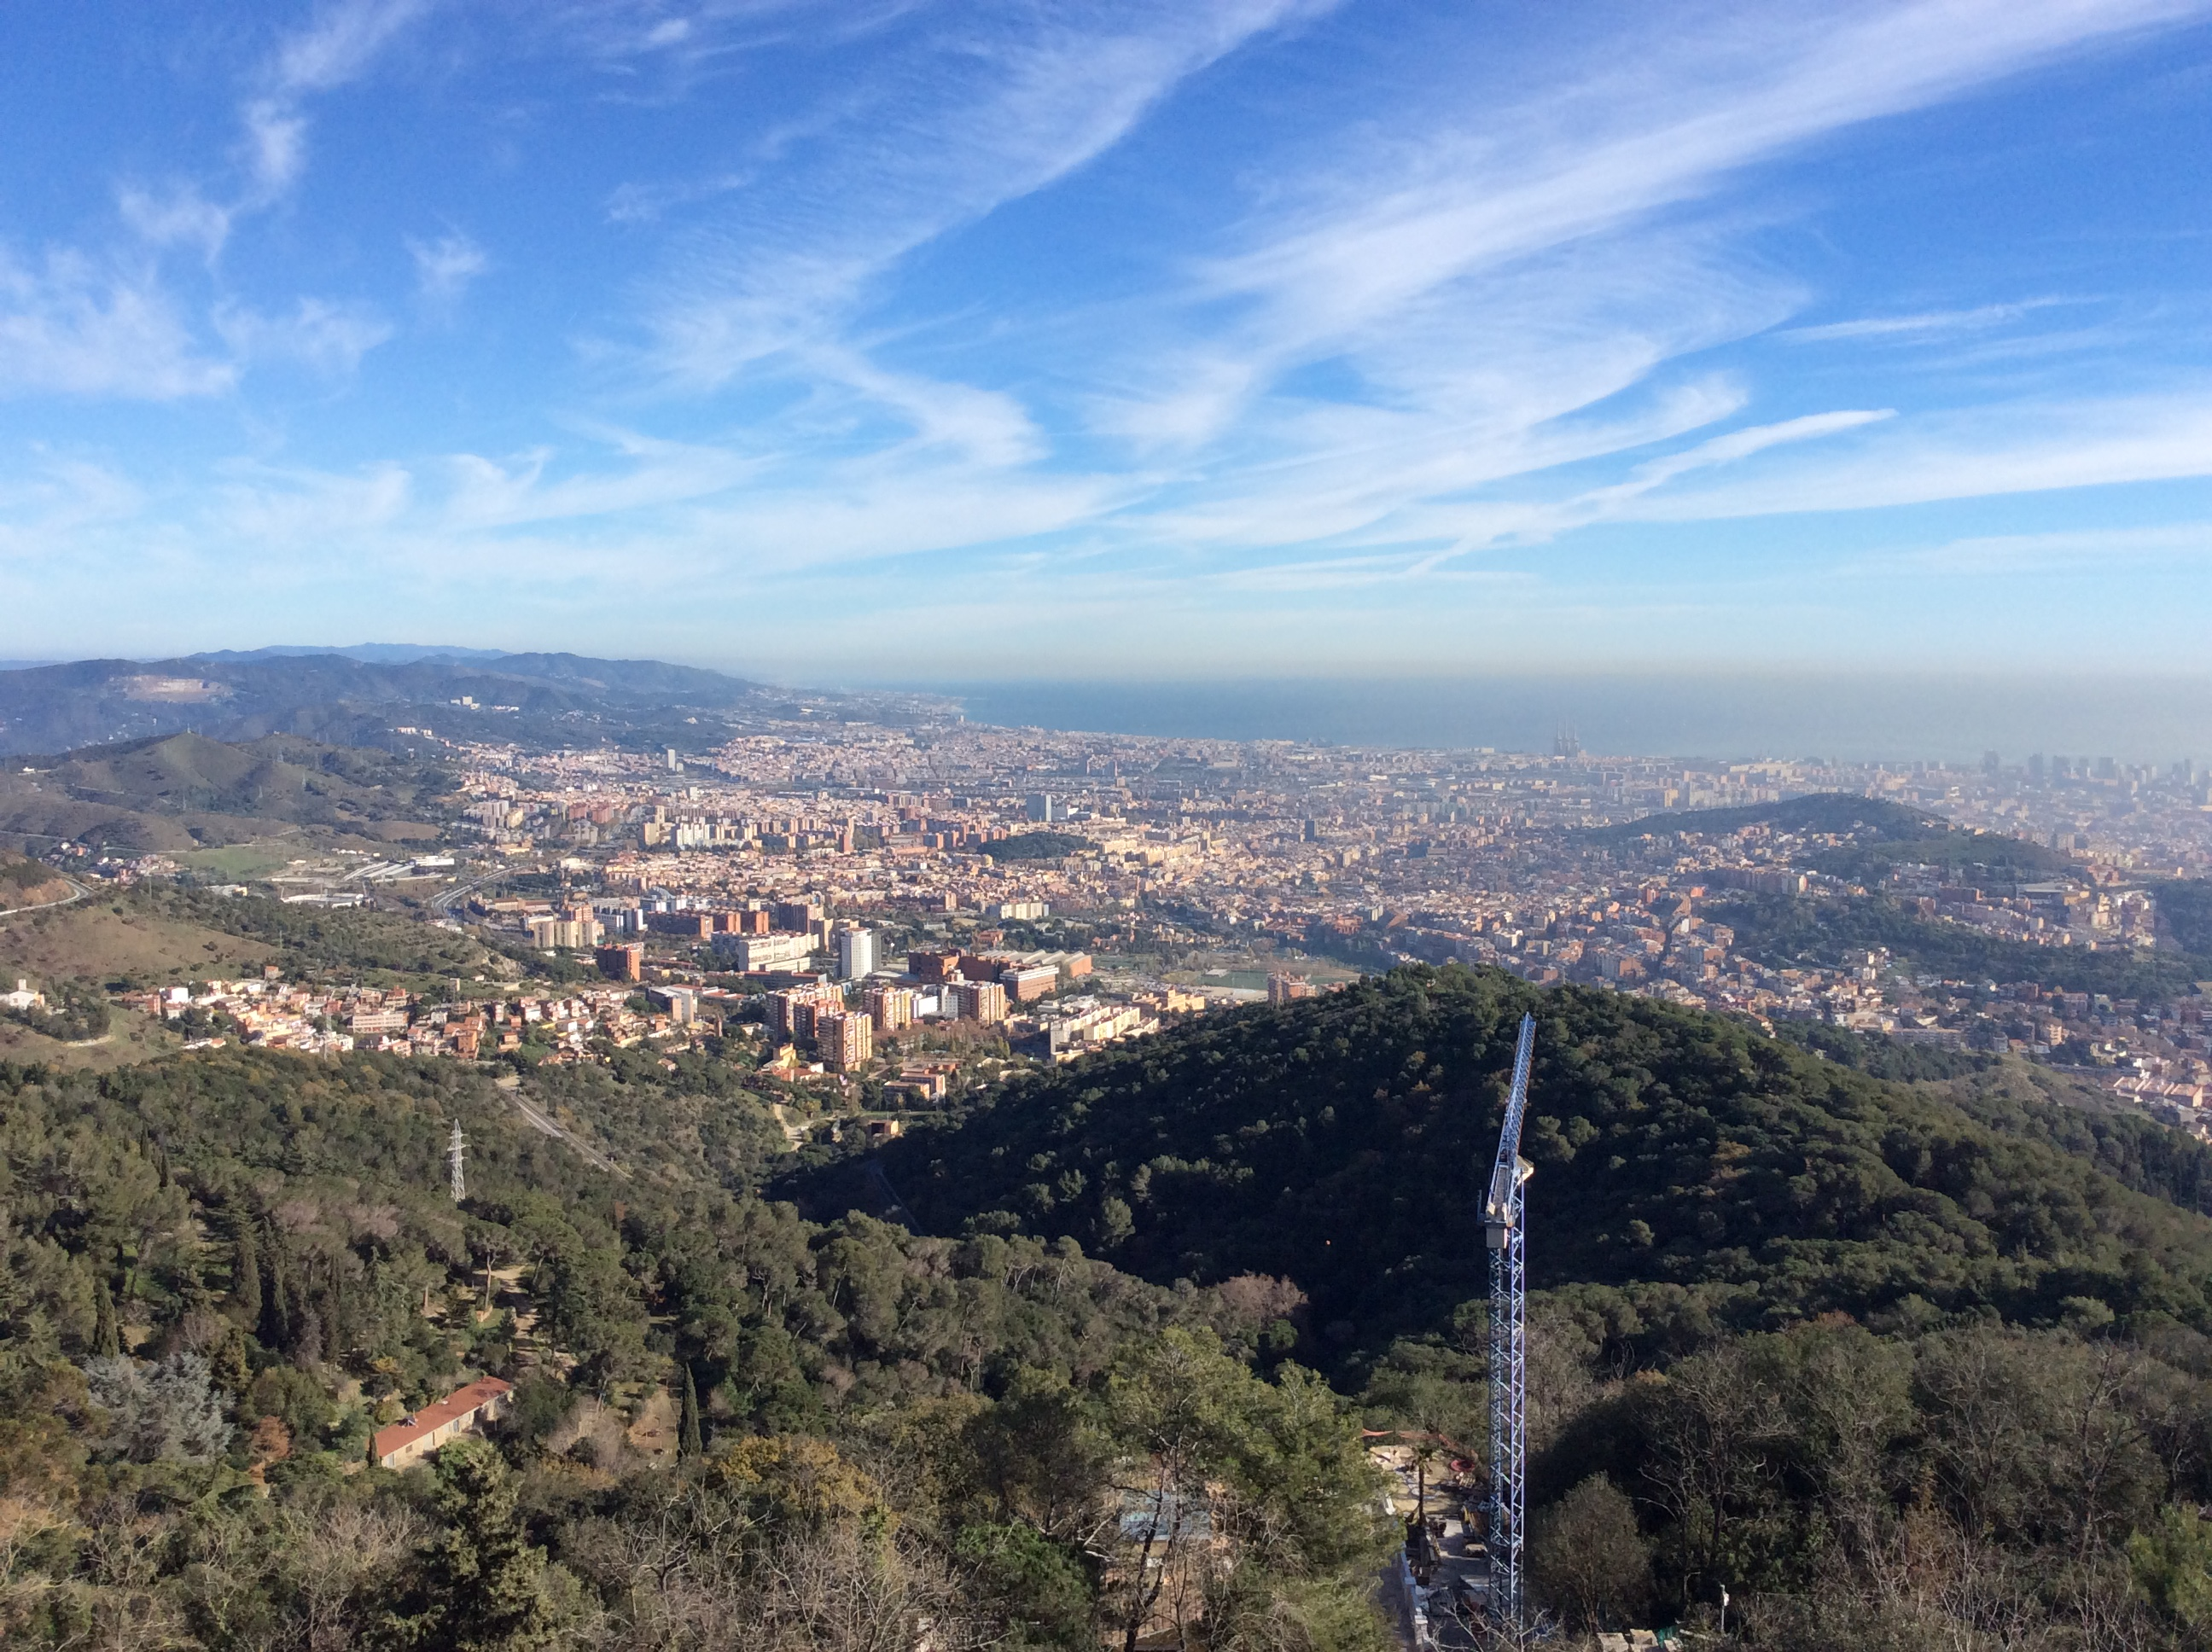
\includegraphics[width=\textwidth]{barc3.jpeg}
        \end{figure}
      \end{column}
      \begin{column}{0.25\textwidth}
        \begin{figure}
          \centering
          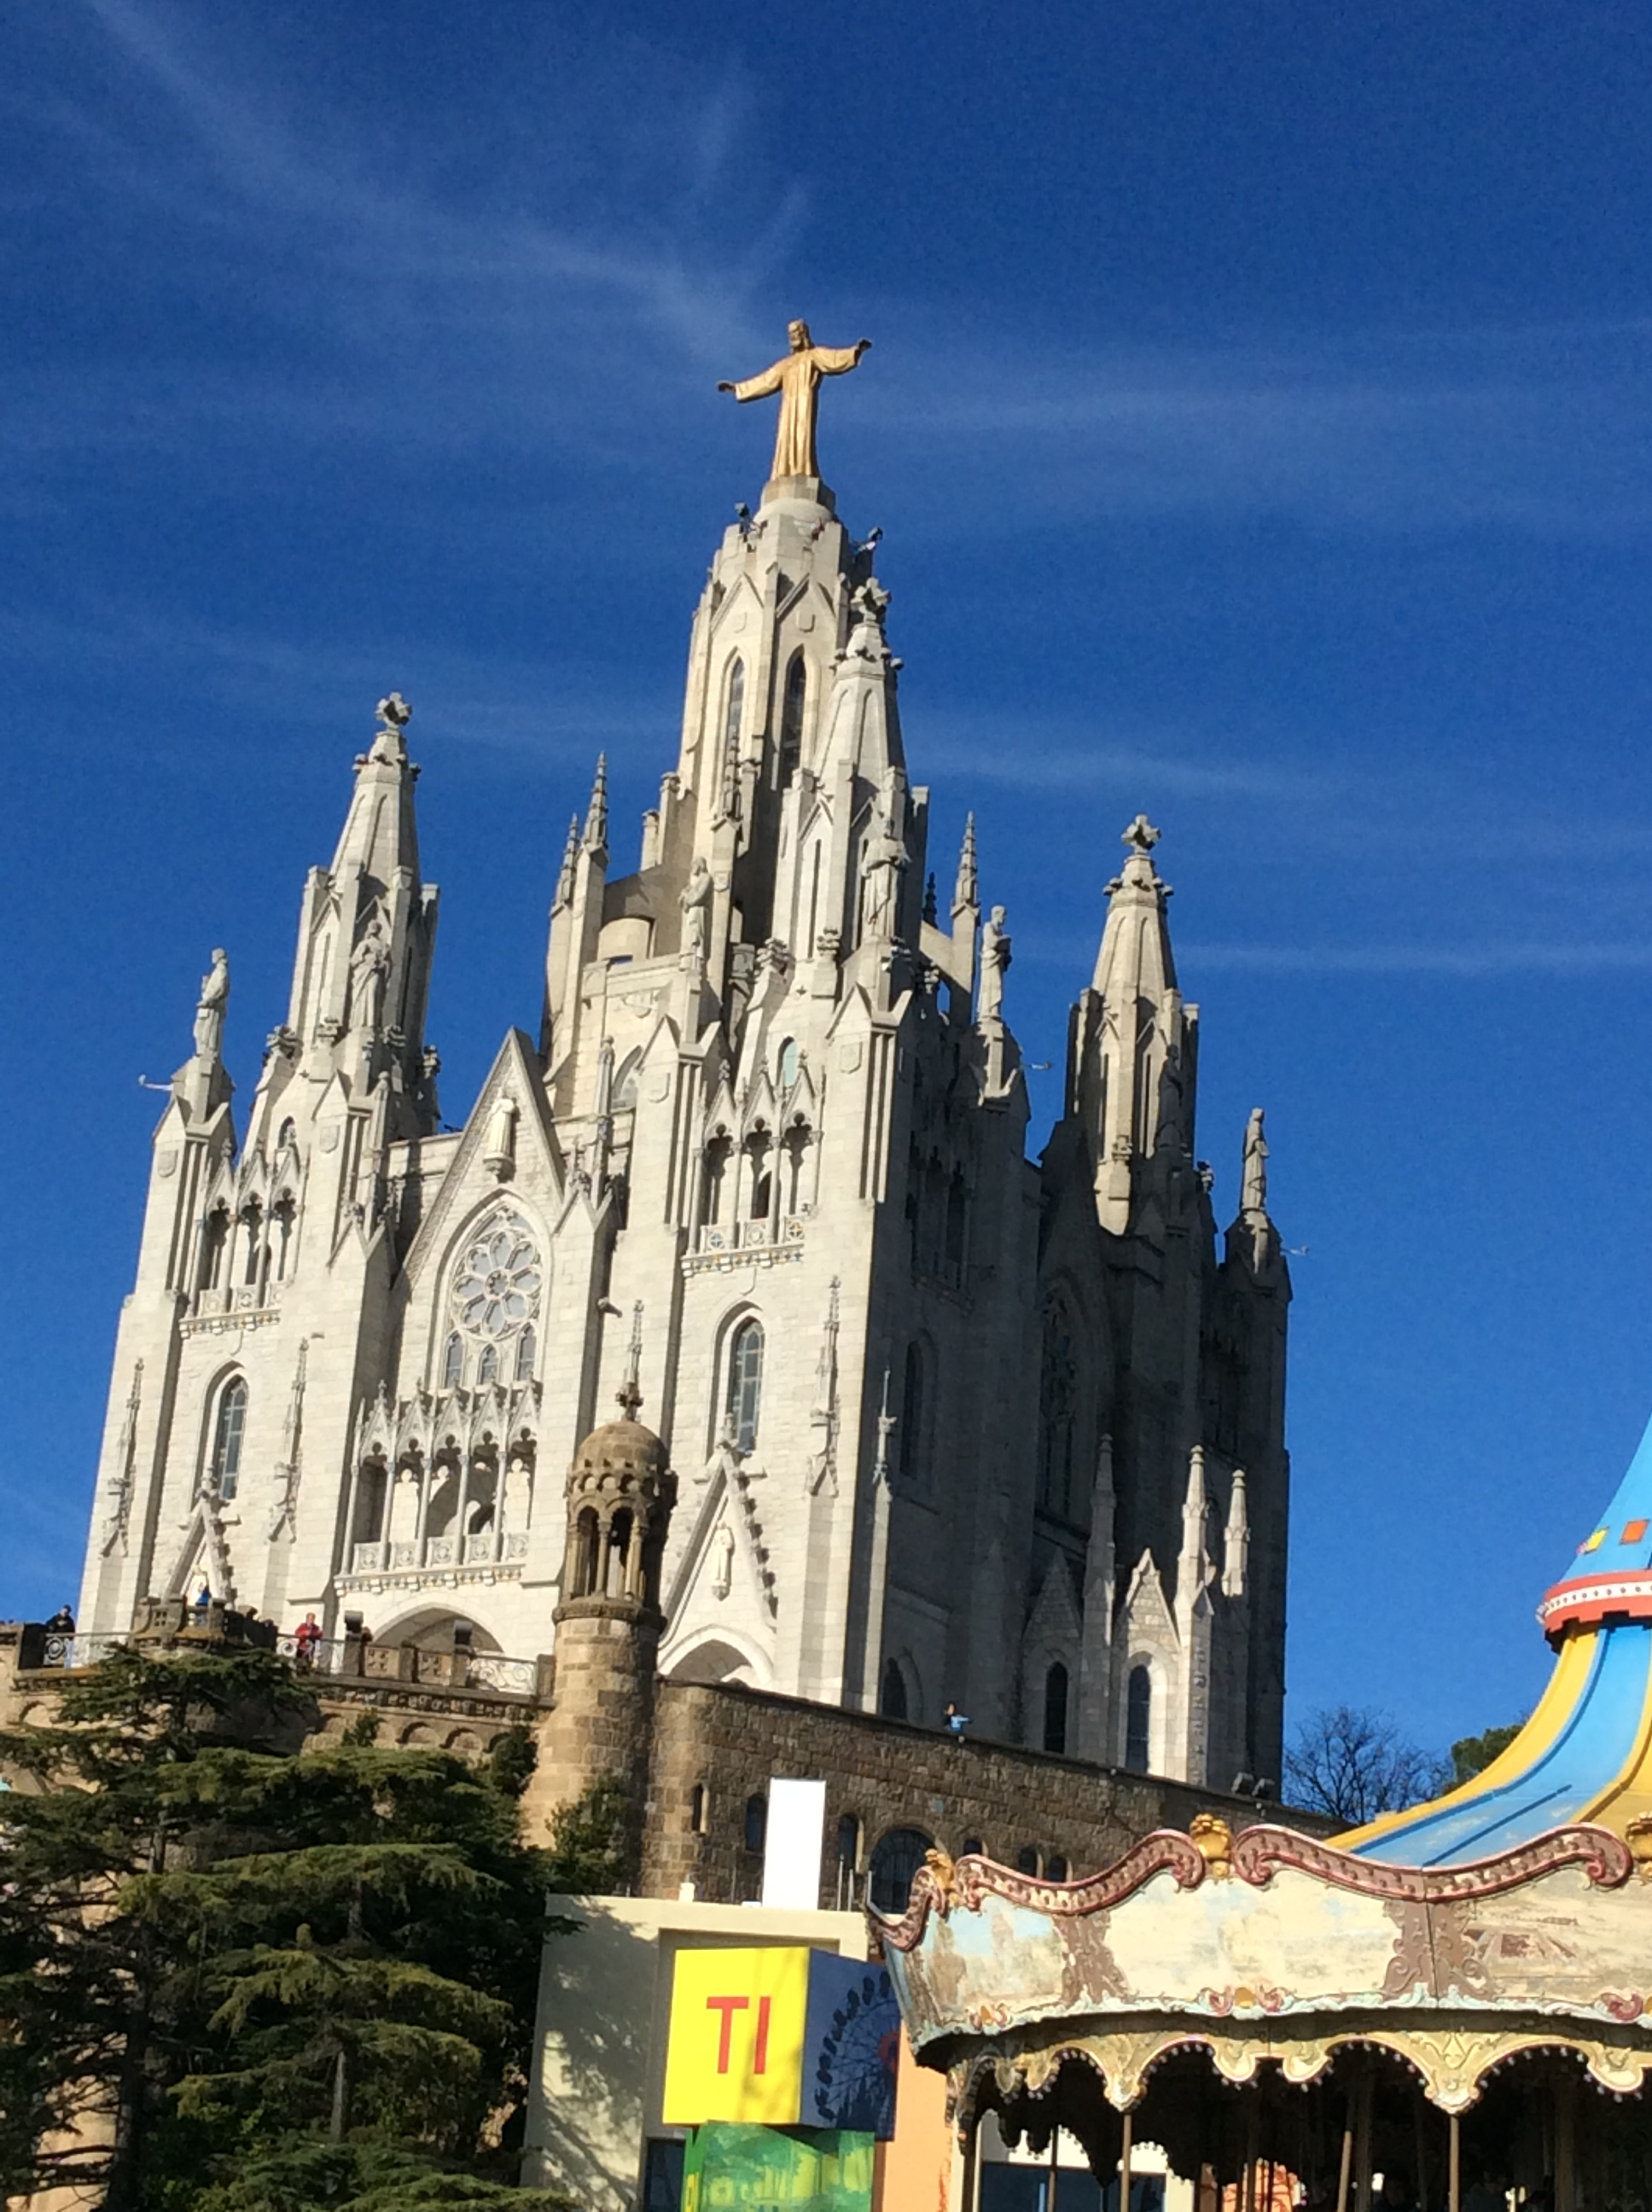
\includegraphics[width=\textwidth]{barc1.jpeg}
        \end{figure}
      \end{column}
      \begin{column}{0.25\textwidth}
        \begin{figure}
          \centering
          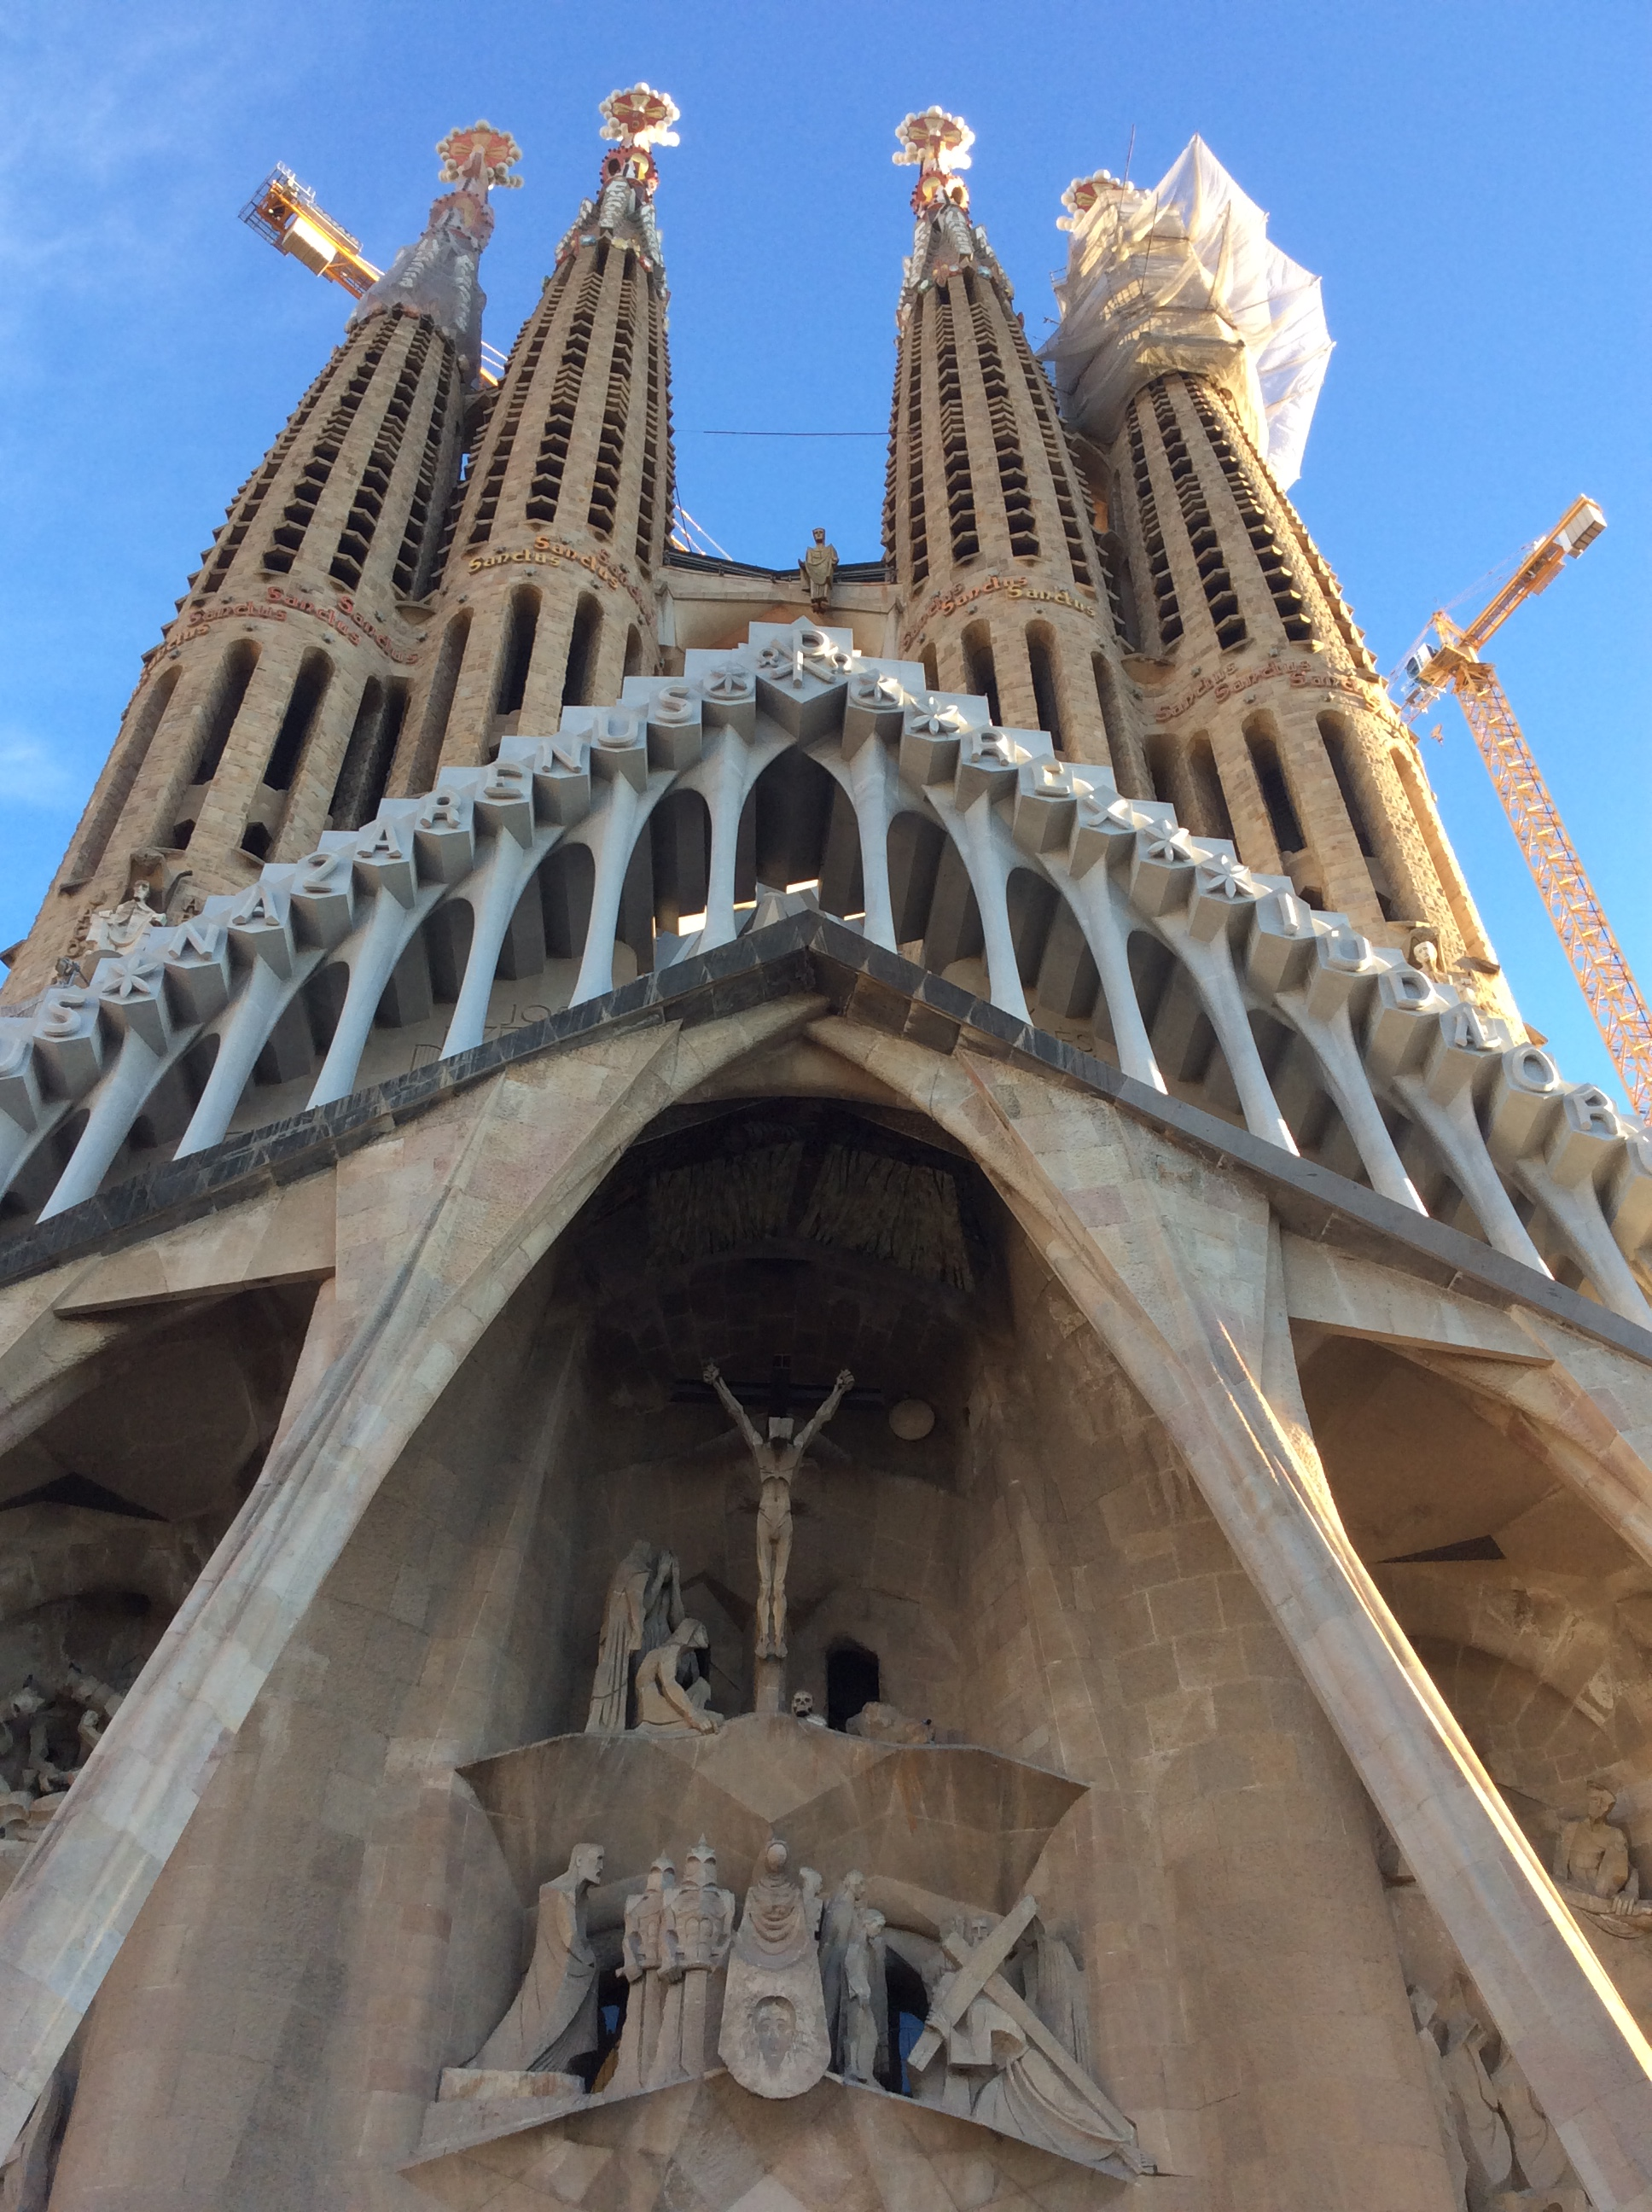
\includegraphics[width=\textwidth]{barc2.jpeg}
        \end{figure}
      \end{column}
    \end{columns}
  \end{frame}

  \begin{frame}[noframenumbering]

    \begin{center}
      \Huge{Thank you!}\\~\\
      \huge{Take home Messages}
      \normalsize
      \begin{itemize}
        \item Deep Learning is no longer just a tool!
        \item Emphasis is changing to General AI and Life long learning
        \item Recurrent Neural Networks are very important!
      \end{itemize}
    \end{center}
  \end{frame}

\end{document}
